\chapter{Wprowadzenie}

\section{Wstęp}

%Tu zawrzeć ogólną bajkę na temat zapotrzebowania na przetwarzanie równoległe...
Pod koniec XX wieku rozwój nauk informatycznych nabrał znacznego rozpędu. Postęp techniczny oraz konkurencja na rynku sprzętu sprawiły, że 
komputery stały się dostępne praktycznie dla każdego, a ich ceny uległy znacznemu obniżeniu. Również wydajność obliczeniowa sprzętu wzrasta praktycznie 
z miesiąca na miesiąc. Dzięki temu na całym świecie rozwinęły się sieci komputerowe. Niższy koszt takich sieci i ich duża dostępność sprawiły, że 
zaczęto je wykorzystywać do wykonywania profesjonalnych obliczeń. Znalazło to zastosowanie w takich problemach obliczeniowych, dla których dane 
można było podzielić i przetwarzać je równolegle na wielu jednostkach sprzętowych. \definicja{Przetwarzanie równoległe} (\english{parallel processing}) 
jest obecnie bardzo popularne i wykorzystywane w takich dziedzinach informatyki jak np.~bazy danych, systemy czasu rzeczywistego, systemy operacyjne. 
Głównym celem wykorzystania przetwarzania równoległego jest dążenie do skrócenia czasu wykonywanych obliczeń. Dzięki rozproszeniu obliczeń 
na wiele jednostek przetwarzających, można uzyskać ich wyniki w czasie znacznie krótszym niż gdyby były one wykonywane sekwencyjnie na 
jednej maszynie. Jednak warunkiem skrócenia czasu przetwarzania jest odpowiedni podział danych i dystrybucja ich do procesorów obliczeniowych. 
Przydziału takiego dokonuje się na podstawie informacji m.in. o prędkości łącz komunikacyjnych, mocy obliczeniowej jednostek przetwarzających oraz dostępnej 
pamięci. Należy jednak pamiętać, że nieodpowiedni podział zadań obliczeniowych może spowodować wzrost czasu przetwarzania zamiast jego redukcji.

\section{Cel i zakres pracy}

%Tu zawrzeć ogólną bajkę na temat zapotrzebowania na programy wspierające przetwarzanie równoległe...
W związku z faktem, że prawidłowy przydział danych do jednostek przetwarzających jest tak istotny, powstało wiele algorytmów, których zadaniem 
jest znalezienie uszeregowania zadań jednorodnych minimalizującego czas przetwarzania. Implementacja kilku takich algorytmów była celem prac 
magisterskich realizowanych w poprzednich latach. Celem poniższej pracy jest projekt i implementacja systemu umożliwiającego wybór i wykonanie 
wybranych algorytmów dla zadanych parametrów wejściowych oraz wizualizację wyników ich działania. Jedną z funkcji systemu będzie właśnie możliwość 
generowania plików z danymi wejściowymi. Wyniki uszeregowania dostępne będą zarówno w postaci tekstowej jak i graficznej (\definicja{wykres Gantta}). 
Algorytmy szeregowania będą dostępne w programie jako biblioteki łączone dynamicznie, co zapewni możliwość jego dalszej rozbudowy i rozszerzania.


\chapter{Szeregowanie zadań jednorodnych}

Na temat problemu szeregowania zadań jednorodnych powstało wiele publikacji. Szczegółowe informacje można znaleźć m.in.~w pozycjach: \cite{znPSl96}, 
\cite{robertazzi} oraz \cite{veeravalli}. Poniżej zostały przedstawione wybrane założenia dotyczące problemu szeregowania.

\section{Definicja zadania jednorodnego}

\definicja{Zadaniem jednorodnym} (\english{divisible job}) nazywać będziemy obliczenia, które można podzielić na części o dowolnym rozmiarze i 
przetwarzać równolegle
na różnych komputerach (procesorach). Przetwarzanie takie może być \definicja{wieloetapowe}, czyli każda jednostka przetwarzająca może otrzymywać dane w wielu 
komunikatach. Założeniem szeregowania zadań jednorodnych jest minimalizacja czasu przetwarzania czyli znalezienie takich rozmiarów paczek 
i sekwencji ich przydziału do procesorów, aby obliczenia zakończyły się jak najszybciej.

\section{Model przetwarzania}\label{model_przetwarzania}

Przyjętym w pracy modelem środowiska rozproszonego jest sieć o topologii gwiazdy (rys.~\vref{rys:arch}). Centralnym elementem tej struktury jest procesor typu 
\definicja{nadzorca} (\english{master, originator}) zwany także \definicja{inicjatorem}. Na początku wszystkie dane, których dotyczą obliczenia, są przechowywane
właśnie na komputerze centralnym.
Jego zadaniem jest rozsyłanie tych danych, które mają zostać przetworzone, oraz ewentualnie zebranie wyników obliczeń. Nadzorca nie zajmuje się przetwarzaniem 
paczek danych. Do tego celu służą \definicja{procesory robocze} (\english{slave}). Procesory przetwarzające nie mogą komunikować się między sobą, natomiast 
procesor centralny może w danej chwili wymieniać informacje tylko z jednym z nich. Istotnym założeniem jest, że procesory robocze mogą jednocześnie odbierać 
paczkę od inicjatora oraz przetwarzać dane otrzymane wcześniej. Jednak do rozpoczęcia przetwarzania każdej paczki niezbędne jest jej całkowite odebranie.
Algorytmy szeregujące mogą przyjmować różne założenia co do szczegółowych cech modelu przetwarzania. Czasami czas zwracania wyników jest 
uznawany za nieistotny i zaniedbywalnie mały, a niekiedy jest on uwzględniany. Podobna sytuacja dotyczy pojemności bufora pamięci. Jeśli 
założymy, że pamięć procesora przetwarzającego jest nieograniczona i może pomieścić przynajmniej jedno całe zadanie, 
%(dla każdego $i$: $\alpha{_i}$$<$$B{_i}$), 
nie zachodzi potrzeba analizy zajętości buforów podczas przesyłania paczek.

\begin{figure}[hbt]
\centering%
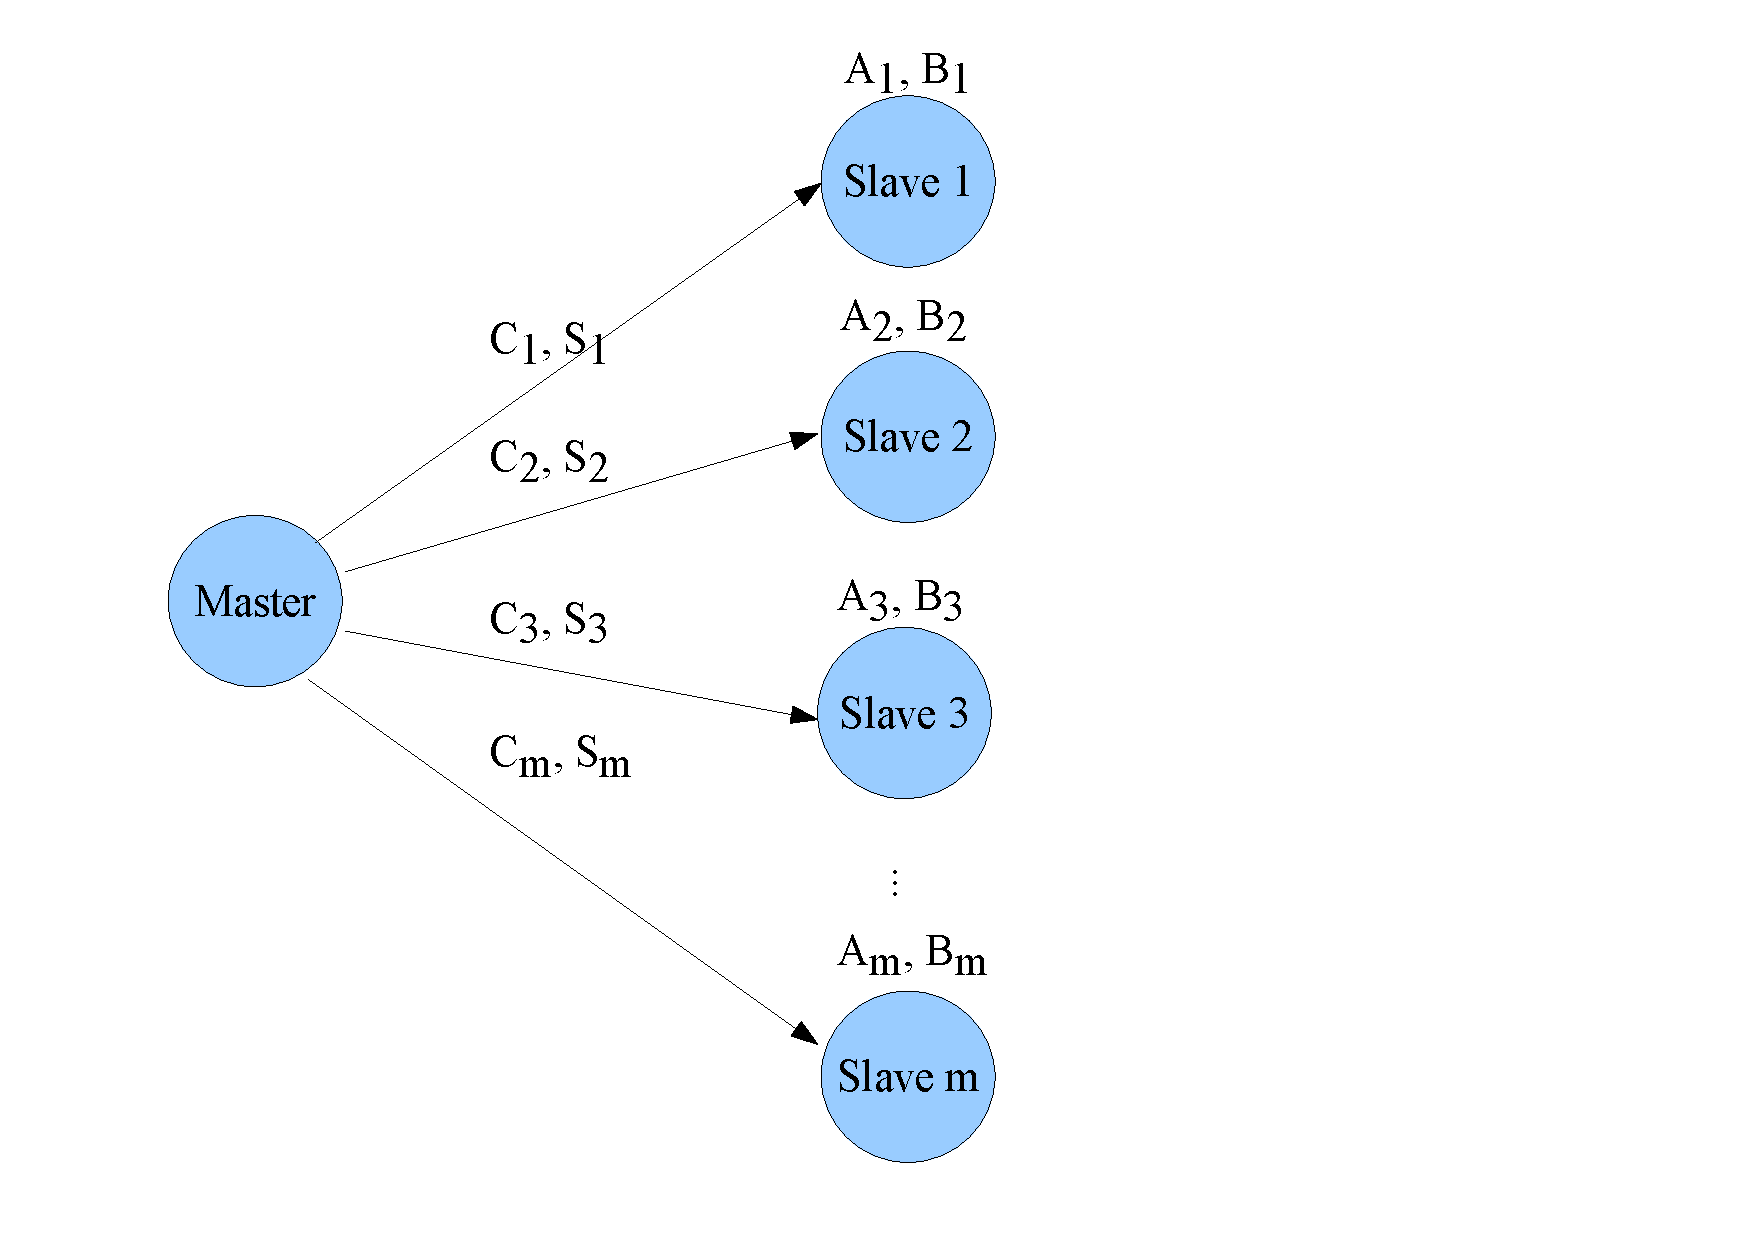
\includegraphics[scale=0.4]{figures/architektura.pdf}
\caption{Architektura sieci rozproszonej.}\label{rys:arch}
\end{figure}

Każdy z procesorów przetwarzających jest opisany przez zbiór następujących wartości:
\begin{itemize}
	\item \textbf{$A_i$} -- odwrotność prędkości przetwarzania $i$-tego procesora,
	\item \textbf{$C_i$} -- odwrotność prędkości łącza pomiędzy inicjatorem a $i$-tym procesorem,
	\item \textbf{$S_i$} -- opóźnienie komunikacyjne łącza pomiędzy inicjatorem a $i$-tym procesorem,
	\item \textbf{$B_i$} -- pojemność bufora pamięci $i$-tego procesora.
\end{itemize}

%\section*{Przykład}
%Jednym z najpowszechniejszych przykładów zadania jednorodnego jest przetwarzanie bazy danych składających się z dużej liczby rekordów. 
%Aby przeszukać taką bazę, możemy przetwarzać dowolne grupy rekordów niezależnie od siebie.

\chapter{Algorytmy}

W tym rozdziale przedstawiono opis algorytmów, które mogą być wykorzystane przez projektowany system.

\section{Algorytmy dokładne}

\definicja{Algorytm dokładny} to metoda, która daje gwarancję na uzyskanie optymalnego rozwiązania dla każdej instancji problemu obliczeniowego (jeśli takie rozwiązanie 
istnieje). Niestety, w większości przypadków, aby otrzymać rozwiązanie optymalne, niezbędne jest przejrzenie całego lub prawie całego zbioru dostępnych 
rozwiązań. Cecha ta jest istotną wadą, ponieważ powoduje wykładniczy czas wykonania algorytmu. W związku z tym dla większych instancji 
może nie być możliwe uzyskanie rozwiązania w akceptowalnym czasie.

Złożoność obliczeniowa algorytmu dokładnego dla problemu szeregowania zadań jednorodnych zależy wykładniczo od liczby procesorów w systemie ($m$)
oraz liczby paczek danych ($n$), które muszą zostać przetworzone.

\subsection{Metoda podziału i ograniczeń}

\definicja{Metoda podziału i ograniczeń} (\english{Branch and Bound}) dąży do zmniejszenia liczby przeszukiwanych rozwiązań, a przez to skrócenie czasu obliczeń. 
Jej działanie polega na uporządkowanym przeszukiwaniu 
zbioru rozwiązań. W związku z tym dokonuje się podziału tego zbioru na pewną liczbę podzbiorów. Każdy z nich jest charakteryzowany przez wartość 
zwaną, w przypadku minimalizacji funkcji celu (tak jak to ma miejsce w problemie szeregowania zadań jednorodnych), \definicja{dolnym ograniczeniem}. 
Oprócz tego, dla całego zbioru rozwiązań należy określić również \definicja{górne ograniczenie}. Jego wartość odpowiada funkcji celu najlepszego znalezionego 
do tej pory rozwiązania. Po każdym podziale następuje sprawdzenie czy wartość dolnego ograniczenia dla otrzymanego podzbioru nie przekracza 
zdefiniowanego ograniczenia górnego.

Jeśli dolne ograniczenie jest większe lub równe górnemu, nie zachodzi potrzeba dalszego podziału i przeglądania tego podzbioru rozwiązań, 
ponieważ mamy pewność, iż w tej gałęzi drzewa nie uda się znaleźć rozwiązania lepszego niż najlepsze znane do tej pory. Dany wierzchołek 
drzewa nie jest już dalej rozwijany. Postępowanie takie nazywa się \definicja{odcięciem} gałęzi drzewa.

W przypadku dojścia do ostatniego wierzchołka w rozwijanej gałęzi drzewa (liścia), należy porównać wartość funkcji celu otrzymanego rozwiązania 
z obecnym górnym ograniczeniem. Jeśli okaże się, że wartość ta jest lepsza (mniejsza) od górnego ograniczenia, oznacza to, że znaleziono lepsze 
rozwiązanie od wszystkich do tej pory znanych. Jako aktualne górne ograniczenie przyjmuje się od tej chwili wartość funkcji celu tego rozwiązania.

Algorytm kończy swe działanie, kiedy zostanie znalezione dopuszczalne rozwiązanie, którego wartość funkcji celu jest nie większa od 
najmniejszego dolnego ograniczenia wszystkich nie podzielonych podzbiorów.

Rozgałęzianie drzewa w przypadku rozwiązywania problemów szeregowania zadań jednorodnych polega na dodawaniu kolejnych węzłów odpowiadających 
procesorom, do których może zostać wysłana paczka danych. Proces ten został zobrazowany na rysunku~\vref{rys:bb-cut}. Liczba wierzchołków w 
nieodciętej gałęzi odpowiada liczbie paczek, które należy rozdysponować i wynosi $n$. Do obliczenia wartości funkcji celu można wykorzystać 
odpowiednio sformułowane zadanie programowania liniowego, które można sformułować następująco:

\vspace{5mm}\noindent
Minimalizować $C_{max}$ przy ograniczeniach:

\begin{equation}\label{eq1}
\sum\limits_{j=1}^{i} (S_{d_j} + \alpha_j C_{d_j}) 
                    + A_{d_i} \sum\limits_{j \epsilon H_i} \alpha_j \le C_{max}   \quad\quad i = 1, \ldots{}, n
\end{equation}
\begin{equation}\label{eq2}
\sum\limits_{i=1}^{n} \alpha_i = V
\end{equation}

\noindent gdzie:\\
$d{_i}$ -- numer procesora, do którego trafia paczka $i$,\\
$H{_i}$ -- zbiór numerów paczek wysłanych do procesora $d{_i}$ poczynając od paczki $i$.
\vspace{5mm}

W pierwszym ograniczeniu czas transmisji paczek $1, \ldots{}, i$ jest wyrażony poprzez sumę:
\begin{displaymath}
\sum\limits_{j=1}^i (S_{d_j} + \alpha_j C_{d_j}), \nonumber
\end{displaymath}
natomiast $A_{d_i} \sum\limits_{j \epsilon H_i} \alpha_j$ wyraża czas obliczeń nad paczkami, które zostały przydzielone do procesora $d{_i}$ 
rozpoczynając od paczki $i$-tej. Ograniczenie~\ref{eq1} daje gwarancję, że żaden procesor nie wykona pracy po czasie bedącym końcem uszeregowania, a 
ograniczenie~\ref{eq2} zapewnia wykonanie całej pracy.

\begin{figure}[t]
\centering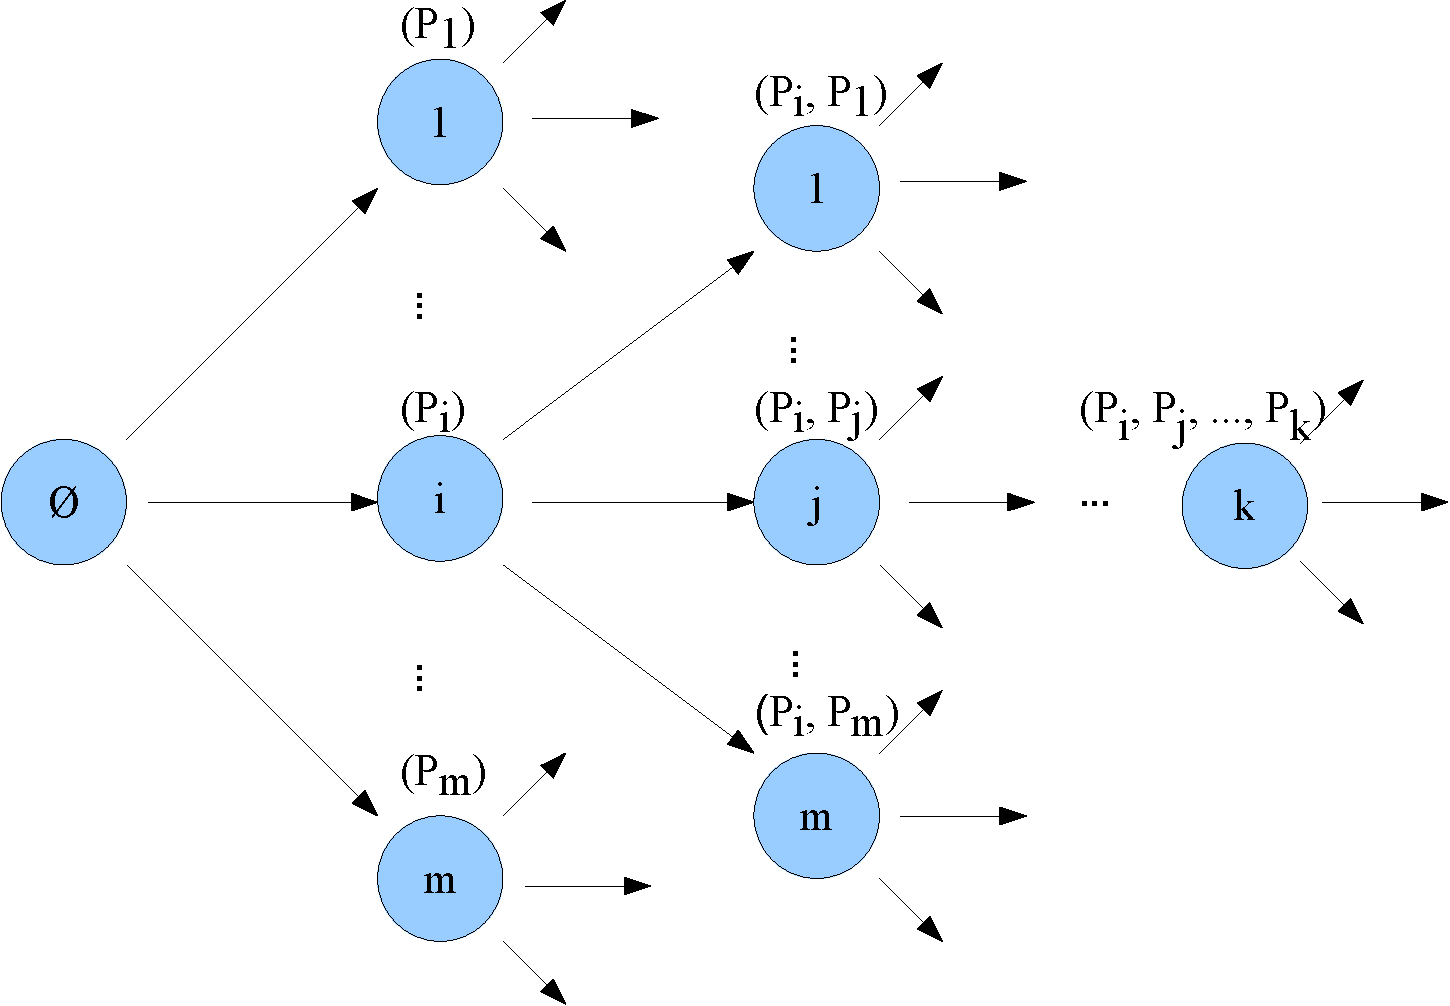
\includegraphics[scale=0.5]{figures/bb1.pdf}
\caption{Rozgałęzianie drzewa w metodzie podziału i ograniczeń.}\label{rys:bb-cut}
\end{figure}

Zasada działania metody podziału i ograniczeń została opisana szczegółowo w publikacji~\cite{bop}. Metoda ta wykorzystana była w pracach magisterskich 
\cite{daniel} oraz \cite{zietkiewicz}.

Wadą rozwiązania jest wykładnicza złożoność tego algorytmu wynosząca w najgorszym przypadku $O(m^n)$.

\section{Algorytmy heurystyczne}

Algorytmy heurystyczne służą m.in.~do rozwiązywania trudnych problemów obliczeniowych w czasie krótszym niż wykładniczy. 
Nie zapewniają one wprawdzie uzyskania optymalnego rozwiązania danego problemu, jednak dzięki skróceniu czasu obliczeń pozwalają 
uzyskać rozwiązanie nierzadko niewiele gorsze od optymalnego, dla takich instancji, dla których algorytm dokładny działałby niedopuszczalnie 
długo. Obecnie dużą popularnością cieszą się metaheurystyki zainspirowane zjawiskami zachodzącymi w przyrodzie lub życiu codziennym. W większości 
przypadków są to algorytmy probabilistyczne.

\subsection{Algorytmy genetyczne}

\definicja{Algorytmy genetyczne} poszukują optimum przetwarzając populację rozwiązań w sposób przypominający ewolucję genomu. W procesie doboru naturalnego 
przeżywają osobniki najlepiej przystosowane do warunków środowiska, w którym żyją. Następnie rozmnażając się przekazują one swoje cechy 
osobnikom potomnym. Dzięki takiemu rozwiązaniu kolejne pokolenia, dzięki genom uzyskanym od rodziców, stają się coraz lepiej przystosowane do 
życia w danym środowisku.

Klasyczna wersja algorytmu genetycznego ma stały, powtarzalny schemat działania (rys.~\vref{rys:genetyczny}). Punktem wyjścia jest zawsze 
stworzenie początkowej populacji osobników. Populacja startowa jest zbiorem chromosomów utworzonych losowo. Następnie za pomocą 
określonych kryteriów z populacji tej wybierane są osobniki (\definicja{selekcja}), 
które będą stanowić podstawę do uzyskania kolejnego pokolenia. Przy udziale operatorów takich jak krzyżowanie i mutacja, 
z osobników rodzicielskich otrzymujemy nową populację, której funkcja przystosowania, dzięki odziedziczonym genom, powinna być 
już wyższa (krótsza długość uszeregowania). Algorytm kończy działanie po osiągnięciu zadanego warunku stopu, np.~maksymalnej 
liczbie iteracji lub maksymalnej liczbie iteracji bez poprawy rozwiązania.

\begin{figure}[t]
\centering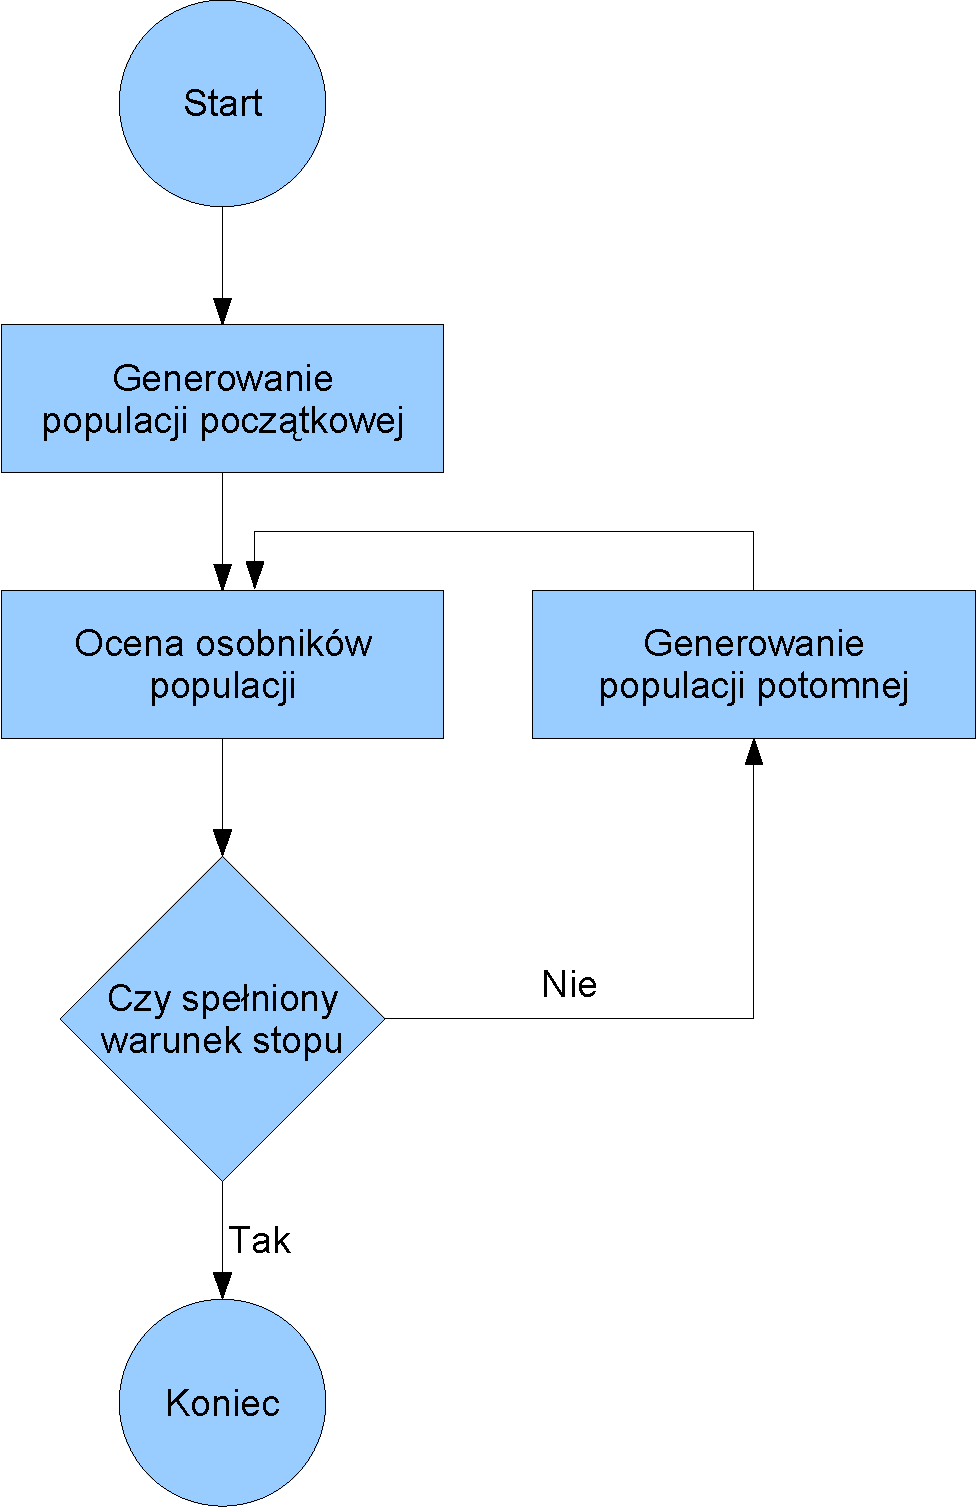
\includegraphics[scale=0.5]{figures/genetyczny_schemat.pdf}
\caption{Schemat działania algorytmu genetycznego.}\label{rys:genetyczny}
\end{figure}

\subsubsection*{Podstawowe pojęcia z dziedziny algorytmów genetycznych}
\begin{enumerate}[a)]
    \item \textbf{Chromosom} -- zakodowane pojedyncze rozwiązanie,
    \item \textbf{Populacja chromosomów} -- zbiór rozwiązań,
    \item \textbf{Gen} -- element chromosomu, cecha, znak w ciągu kodowym rozwiązania,
    \item \textbf{Allel} -- wariant cechy.
\end{enumerate}

\subsubsection*{Operatory genetyczne}
\begin{enumerate}[a)]
    \item \textbf{Selekcja} -- Celem selekcji jest wybranie z populacji osobników o najlepszej funkcji przystosowania. Osobniki te poddane zostaną 
	później krzyżowaniu i mutacji w celu wygenerowania następnej populacji rozwiązań. Istnieje kilka sposobów wyboru chromosomów, przedstawione zostaną 
	najczęściej używane:
		\begin{itemize}
			\item \textbf{Metoda ruletki} -- Cała populacja odwzorowana jest w postaci koła ruletki. Każdemu osobnikowi odpowiada wycinek koła odpowiedni do jego 
			funkcji przystosowania (im lepsza wartość funkcji, tym większy wycinek koła). Wybór $n$ chromosomów polega na $n$-krotnym zakręceniu kołem ruletki. 
			Dzięki takiej metodzie osobniki o lepszej funkcji przystosowania mają większe szanse wybrania.
			\item \textbf{Ranking} -- Dla każdego chromosomu obliczana jest jego funkcja przystosowania. Następnie osobniki są sortowane od najlepszego 
			do najgorszego, wg obliczonej funkcji. Do dalszych operacji wybrane zostają osobniki z początku listy.
			\item \textbf{Metoda turniejowa} -- Z populacji wybieranych jest kilka osobników. Najlepszy z nich wchodzi w skład grupy rodzicielskiej. Operacja 
			ta jest powtarzana do uzyskania populacji rodziców o zadanym rozmiarze.
		\end{itemize}
    \item \textbf{Krzyżowanie} -- Operacja ta polega na wymianie informacji między dwoma osobnikami z grupy rodzicielskiej. 
	Rezultatem są dwa osobniki potomne, które wejdą w skład kolejnej populacji. Wymiana materiału genetycznego chromosomów wybranych w procesie selekcji 
	sprawia, że niektórzy potomkowie mają lepszą funkcję przystosowania niż ich rodzice. Zazwyczaj krzyżowaniu podlega tylko część populacji 
	rodziców wybrana z pewnym prawdopodobieństwem zwanym prawdopodobieństwem krzyżowania. Pozostałe osobniki z grupy rodziców przechodzą niezmienione 
	do nowej populacji potomnej. Istnieją różne metody krzyżowania:
		\begin{itemize}
			\item \textbf{Krzyżowanie jednopunktowe} -- losowany jest jeden punkt krzyżowania, który dzieli każdego rodzica na dwie części, następnie zachodzi wymiana 
			fragmentu materiału genetycznego między chromosomami rodzicielskimi. W zależności od tego czy punkt krzyżowania wybrany był wspólny dla 
			obu rodziców, czy też różny dla każdego, osobniki potomne mogą mieć identyczną bądź różną długość.
			\item \textbf{Krzyżowanie wielopunktowe} -- chromosomy rodzicielskie ulegają podziałowi na kilka części, osobniki potomne powstają wskutek przeplatania 
			materiału genetycznego pochodzącego od rodziców.
		\end{itemize}
    \item \textbf{Mutacja} -- W przeciwieństwie do krzyżowania, mutacja jest operacją przeprowadzaną na jednym chromosomie. Najczęściej polega ona po prostu 
	na losowej zmianie wartości jednego wybranego genu (aczkolwiek podobnie jak krzyżowanie może dotyczyć większej liczby genów z chromosomu). Mutacja
	zachodzi z pewnym prawdopodobieństwem zwanym prawdopodobieństwem mutacji, jego wartość jest zazwyczaj bardzo mała. Zadaniem tej operacji 
	jest zapewnienie zmienności chromosomów w populacji.
\end{enumerate}

\subsubsection*{Algorytmy genetyczne a szeregowanie zadań jednorodnych}
Dla problemu szeregowania zadań jednorodnych każdy osobnik w populacji reprezentuje pojedyncze uszeregowanie. Gen w chromosomie odpowiada 
numerowi procesora, do którego jest wysyłana paczka danych. Ułożenie genów osobnika odzwierciedla kolejność przydziału paczek do procesorów.

Tematykę użycia algorytmów genetycznych w szeregowaniu zadań jednorodnych opisuje publikacja~\cite{div_ga1}. Algorytm znajdujący rozwiązanie dla 
problemu szeregowania zadań został przedstawiony w pracy~\cite{rogala}.

\subsection{Przeszukiwanie lokalne}

\definicja{Lokalne przeszukiwanie} jest algorytmem heurystycznym, który można stosować, gdy zależy nam na bardzo szybkim otrzymaniu rozwiązania. 
Pozwala on znaleźć rozwiązanie problemu w czasie często jeszcze krótszym niż opisane wcześniej algorytmy genetyczne, wymaga również 
mniejszych zasobów pamięciowych. Algorytm ten opiera się na pojęciu sąsiedztwa, które w najprostszy sposób można określić jako zbiór rozwiązań 
podobnych do bieżącego. Pierwszy krok przeszukiwania lokalnego polega na wygenerowaniu pojedynczego rozwiązania startowego. Rozwiązanie to 
może być utworzone losowo lub według jakiegoś algorytmu. W kolejnych krokach algorytm iteracyjnie przeszukuje jego sąsiedztwo. Wybór kolejnego 
rozwiązania zależy od przyjętej strategii:
\begin{itemize}
	\item \textbf{Strategia zachłanna} -- podczas przeszukiwania sąsiedztwa wybierane jest pierwsze rozwiązanie, które ma lepszą funkcję celu od bieżącego.
	\item \textbf{Strategia stroma} -- następuje przeszukanie wszystkich rozwiązań z sąsiedztwa, a następnie wybór tego, które funkcję celu poprawia najbardziej.
\end{itemize}

Zakończenie działania algorytmu ma miejsce, gdy w zbiorze sąsiadów bieżącego rozwiązania nie ma takiego, który poprawiałby funkcję celu.

\begin{figure}[t]
\begin{center}
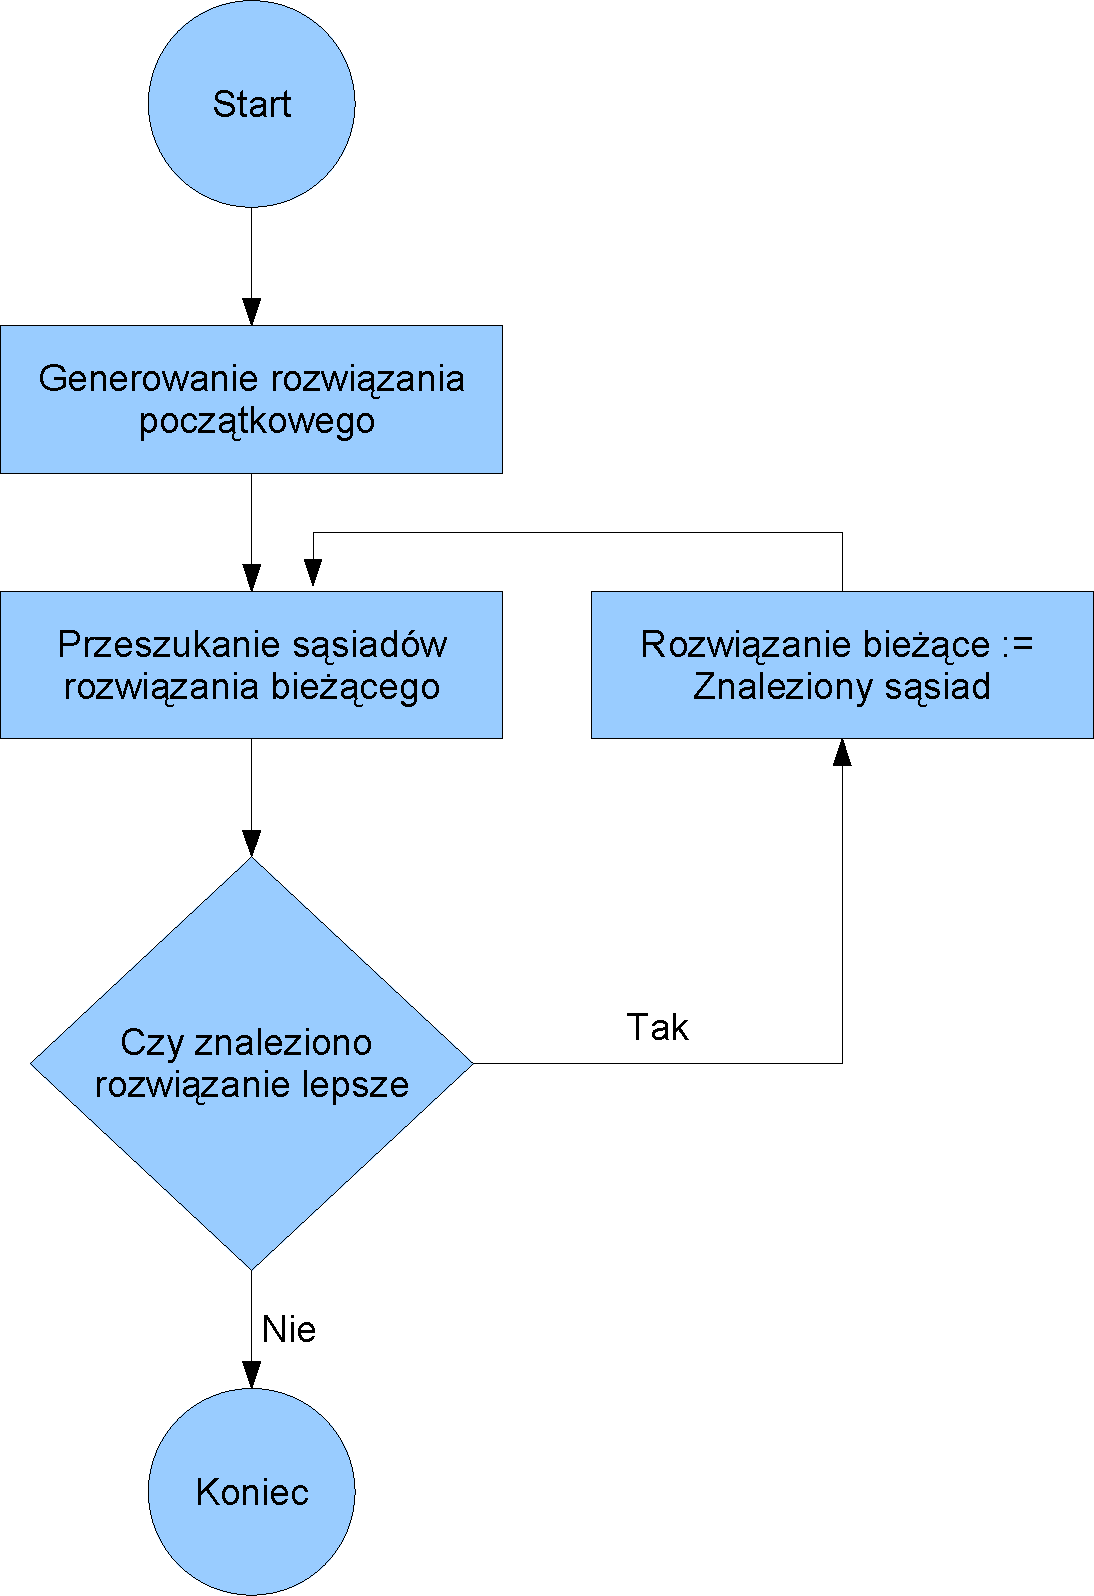
\includegraphics[scale=0.5]{figures/ls_schemat.pdf}
\end{center}
\caption{Schemat działania algorytmu przeszukiwania lokalnego.}\label{rys:ls}
\end{figure}

Wadą algorytmu przeszukiwania lokalnego jest to, że bardzo często znajduje on tylko optimum lokalne. Aby chociaż w pewnym stopniu wyeliminować 
ten problem, stosuje się metodę \akronim{GRASP} (\english{Greedy Randomized Adaptive Search Procedure}), czyli  wielokrotne uruchomienie algorytmu 
z losowym rozwiązaniem początkowym. Inną możliwością jest akceptacja pewnych pogorszeń funkcji celu (aby podjąć próbę wyjścia z optimum 
lokalnego) lub zastosowanie definicji sąsiedztwa takiej, że algorytm przeszukiwał będzie większą część rozwiązań dopuszczalnych.

\subsection{Symulowane wyżarzanie}

\definicja{Symulowane wyżarzanie} należy do grupy algorytmów przeszukiwania globalnego. Algorytm ten wzorowany jest na metodach stosowanych w metalurgii. 
Działanie jego odwzorowuje takie procesy jak rozgrzewanie metalu a następnie powolne, stopniowe schładzanie go w celu osiągnięcia krystalizacji materiału.
Podobnie jak w przeszukiwaniu lokalnym na początku mamy do dyspozycji pewne rozwiązanie startowe, następnie iteracyjnie w każdym kroku 
wybierane zostaje rozwiązanie kolejne, bliższe optymalnemu. Wybór kolejnego rozwiązania zależy oczywiście od stanu bieżącego. Jeśli funkcja celu 
proponowanego stanu, jest lepsza od aktualnej, kandydujące rozwiązanie staje się aktualnym. Jednak gorsza wartość tej funkcji wcale nie musi 
oznaczać odrzucenia rozwiązania. Na podstawie pewnego parametru zwanego temperaturą (analogicznie do rzeczywistego procesu wyżarzania) oraz 
różnicy wartości funkcji celu stanu bieżącego i proponowanego wyliczane jest wtedy prawdopodobieństwo zaakceptowania rozwiązania gorszego:
\begin{displaymath}
P(\Delta{E}) = \frac{1}{c} e^{-\frac{\Delta{E}}{k \cdot T}}
\end{displaymath}
gdzie $c$ to stała normalizująca prawdopodobieństwo po $\Delta{E}$ do $1$, a $k$ to stała Boltzmana.

Takie podejście pozwala na uniknięcie niebezpieczeństwa pozostania w optimum lokalnym. Wartość parametru temperatury jest obniżana, co oznacza, 
że z upływem czasu akceptacja gorszego rozwiązania odbywa się z coraz mniejszym prawdopodobieństwem. Algorytm kończy działanie, kiedy stan 
zostaje ustabilizowany i nie ma już możliwości przejścia do innego rozwiązania. W praktyce oznacza to, że wykonana zostanie pewna założona 
liczba próbnych ruchów bez poprawy jakości rozwiązania.

\subsection{Przeszukiwanie tabu}

\definicja{Metoda tabu} jest metodą poszukiwania rozwiązania w kierunku największego spadku i najmniejszego wzrostu wartości funkcji celu (minimalizacja). 
Jedną z cech algorytmu przeszukiwania tabu jest wykorzystanie pamięci o wykonanych ruchach. Metoda ta rozszerza przeszukiwanie lokalne w tym sensie, 
że kiedy osiągnięte zostanie optimum lokalne, to zaakceptowane zostaje sąsiednie rozwiązanie, które w najmniejszym stopniu pogarsza jakość 
funkcji celu. Aby uniknąć cyklicznych powrotów do minimum lokalnego, stosuje się tzw. listę tabu, która jest kolejką zabronionych ruchów.

Charakterystyczne elementy metody przeszukiwania tabu to:
\begin{itemize}
	\item \textbf{Lista tabu} -- lista ruchów zakazanych. Przejście z jednego rozwiązania do drugiego może być włączone do listy tabu, jeśli ruch ten został 
	ostatnio wykonany lub też był wykonywany zbyt często.
	\item \textbf{Kryterium aspiracji} -- określa kiedy ruch może być usunięty z listy tabu. Najczęściej ograniczenie tabu zostaje usunięte, gdy dzięki 
	temu uzyskamy rozwiązanie lepsze od dotychczasowych.
\end{itemize}

\subsection{Algorytmy mrówkowe}

\definicja{Algorytmy mrówkowe} to kolejny przykład metody rozwiązywania problemów kombinatorycznych zainspirowanej zjawiskami zachodzącymi w przyrodzie. 
Są on analogią do zachowania kolonii mrówek wędrującej do źródła pożywienia. Na przykład gdy takiej drodze zostanie napotkana przeszkoda, którą 
należy ominąć, mrówki idące na przedzie nie będą jeszcze posiadać informacji o tym, która ścieżka jest krótsza. W związku z tym wybór będzie losowy -- 
część pójdzie w prawo, część w lewo. Jednak każda z mrówek będzie pozostawiać za sobą ślad w postaci feromonu, który z upływem czasu traci moc. 
Dzięki temu po dojściu do przeszkody kolejne mrówki skierują się w stronę, gdzie pozostawiony ślad był silniejszy, a więc droga omijająca 
była przeszkodę krótsza.

W algorytmach mrówkowych symulowany jest proces pozostawiania feromonu. Dzięki wielokrotnemu uruchomieniu algorytmu możliwe jest zidentyfikowanie 
optymalnej ścieżki.


\chapter{Projekt systemu}

Rozdział ten opisuje założenia jakie zostały przyjęte odnośnie realizowanej funkcjonalności systemu, a także schematy jego działania oraz 
formaty danych.

\section{Funkcjonalność systemu}

Podstawowym zadaniem systemu jest zebranie kilku algorytmów szeregowania zadań jednorodnych, wybór i wykonanie odpowiedniego algorytmu 
dla pewnych danych wejściowych. Wybór odbywa się na podstawie preferencji użytkownika oraz dostępnych danych wejściowych. Użytkownik ma 
możliwość wybrania algorytmu z listy dostępnych w systemie. Wynikiem działania systemu jest uszeregowanie zadań jednorodnych na podstawie 
wprowadzonych parametrów. Uszeregowanie to może być przedstawione tekstowo lub graficznie (za pomocą wykresu Gantta).

Wspomniane algorytmy były wcześniej zaimplementowane jako osobne programy oraz skompilowane za pomocą różnych kompilatorów (m.in.~Borland C++, 
Microsoft Visual C++). Jednym z zadań wchodzących w skład pracy było ujednolicenie tych programów tak, aby były one napisane z wykorzystaniem 
obiektowości, implementowały jeden wspólny interfejs oraz kompilowały się za pomocą kompilatora MinGW (podrozdział~\vref{mingw}). Takie 
założenie było niezbędne, aby przy wykorzystaniu środowiska Qt zbudować z nich tzw.~wtyczki (\english{plugins}) czyli biblioteki ładowane dynamicznie podczas działania 
systemu. Rysunek~\vref{rys:schemat_main} ilustruje ogólny schemat działania aplikacji.

\begin{figure}[t]
\begin{center}
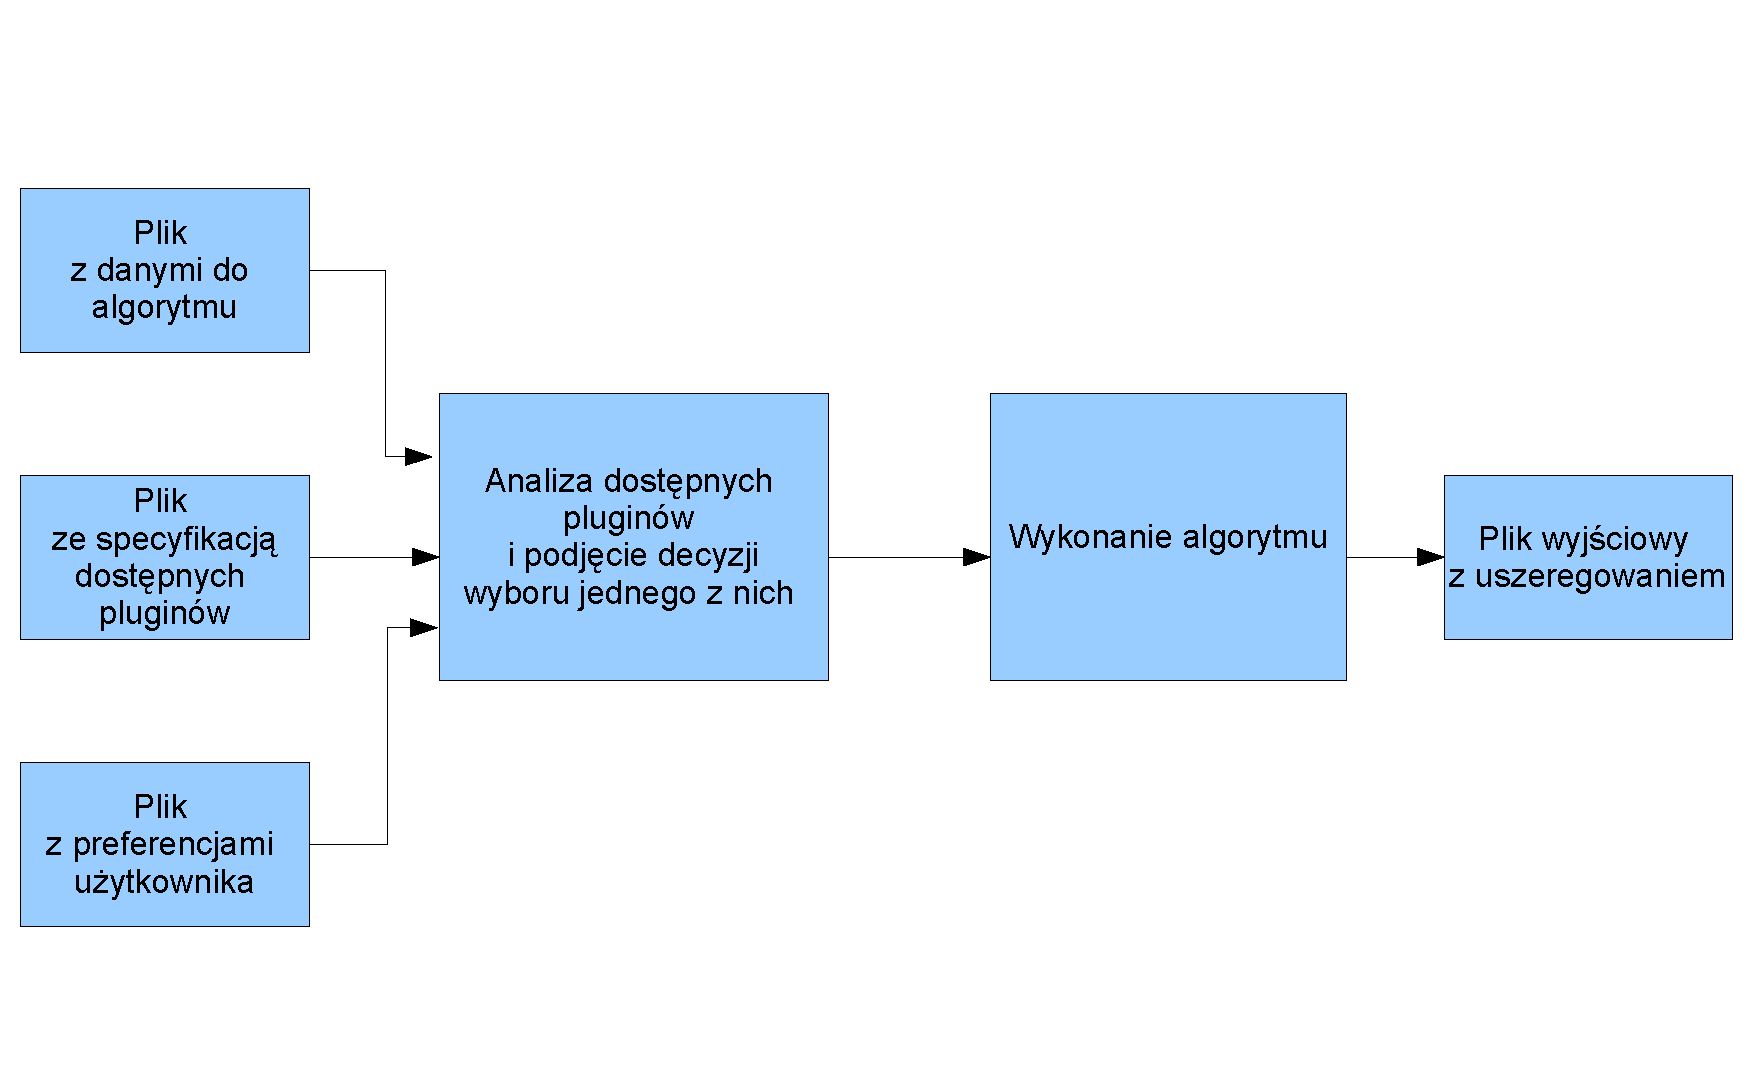
\includegraphics[scale=0.5]{figures/schemat_main.pdf}
\end{center}
\caption{Ogólny schemat działania aplikacji.}\label{rys:schemat_main}
\end{figure}

Dane wejściowe są wczytywane do programu w postaci plików XML. Ich format jest opisany dalej w rozdziale~\vref{pliki}. System udostępnia użytkownikowi 
funkcję wygenerowania takich plików z poziomu programu. Menu oferuje opcje stworzenia następujących plików:
\begin{itemize}
	\item dane procesorów,
	\item dane wtyczek,
	\item preferencje użytkownika.
\end{itemize}
Wybór takiej opcji powoduje uruchomienie okna kreatora pliku, który umożliwia wprowadzenie wszystkich wymaganych wartości, a następnie zapisanie ich 
w postaci pliku XML w wybranej przez użytkownika lokalizacji.

W dalszym działaniu system oferuje użytkownikowi dwie ścieżki wykonania:
\begin{enumerate}[a)]
	\item \label{path1}Wczytanie wyżej wymienionych 3 plików wejściowych powoduje ich weryfikację, a następnie -- gdy są poprawne -- analizę algorytmów dostępnych 
	dla zadanych parametrów. W kolejnym kroku użytkownik ma możliwość wyboru jednej z wtyczek i uruchomienie funkcji obliczającej uszeregowanie. 
	Jeśli wybrany algorytm znalazł rozwiązanie dla problemu szeregowania, to w menu uaktywniane są opcje wyświetlania wyników. Rezultaty działania 
	algorytmu mogą być prezentowane w postaci tekstowej. W takim przypadku system umożliwia ich zapis do pliku w formacie TXT w postaci takiej, 
	jak zostały wyświetlone lub też do pliku o rozszerzeniu \texttt{xml}, gdzie uszeregowanie przedstawione zostaje w postaci znaczników XML. Drugą opcją w menu jest wizualizacja 
	rezultatów szeregowania w postaci wykresu Gantta. Wykres ten ilustruje dystrybucję kolejnych paczek danych do poszczególnych procesorów 
	przetwarzających. Użytkownik ma możliwość zapisu wykresu jako plik graficzny w formacie JPG.
	\item \label{path2}Wejście do programu stanowić mogą też 2 pliki XML -- plik z danymi procesorów oraz plik zawierający gotowe uszeregowanie (będący wynikiem 
	wynikiem działania algorytmu szeregowania). Po ich wczytaniu oraz weryfikacji poprawności dla użytkownika dostępna staje się funkcja 
	wyświetlenia wykresu Gantta.
\end{enumerate}

\subsection*{Ocena i porównywanie algorytmów}

Jak wskazuje tytuł pracy magisterskiej zakładanym celem powstałej aplikacji była możliwość oceny i porównywania działania różnych algorytmów 
szeregowania zadań jednorodnych. Ta funkcjonalność została zrealizowana poprzez opcje wyświetlania i zapisu wyników, jakie zostały zwrócone 
przez metody znajdujące końcowe uszeregowanie. Użytkownik wyświetlając rezultaty tekstowe obserwuje nie tylko przydział poszczególnych paczek danych 
do procesorów, ale również (jeśli konkretna wtyczka udostępnia takie dane) wyniki pośrednie działania algorytmu (np.~w przypadku algorytmu genetycznego 
mogą być to takie informacje jak: liczba popraw, liczba krzyżowań, mutacji, numer wybranej populacji, itp.). Porównanie działania algorytmów 
może być dokonane przy wykorzystaniu funkcji zapisu wyników do plików tekstowych oraz graficznych. Po stworzeniu zbioru uszeregowań oraz 
informacji otrzymanych po wykonaniu wybranych algorytmów na jego podstawie łatwo jest już wykonać porównanie ich efektywności i skuteczności 
w znajdowaniu uszeregowania i minimalizacji funkcji celu.

\section{Schematy blokowe}

Poniższe schematy ilustrują przepływ sterowania w programie. Przedstawiono na nich najważniejsze możliwe ścieżki uruchomienia.

\begin{itemize}
	\item Główna ścieżka wykonania programu (podpunkt~\vref{path1}), rys.~\vref{rys:schemat1}.
		\begin{figure}[p]
		\centering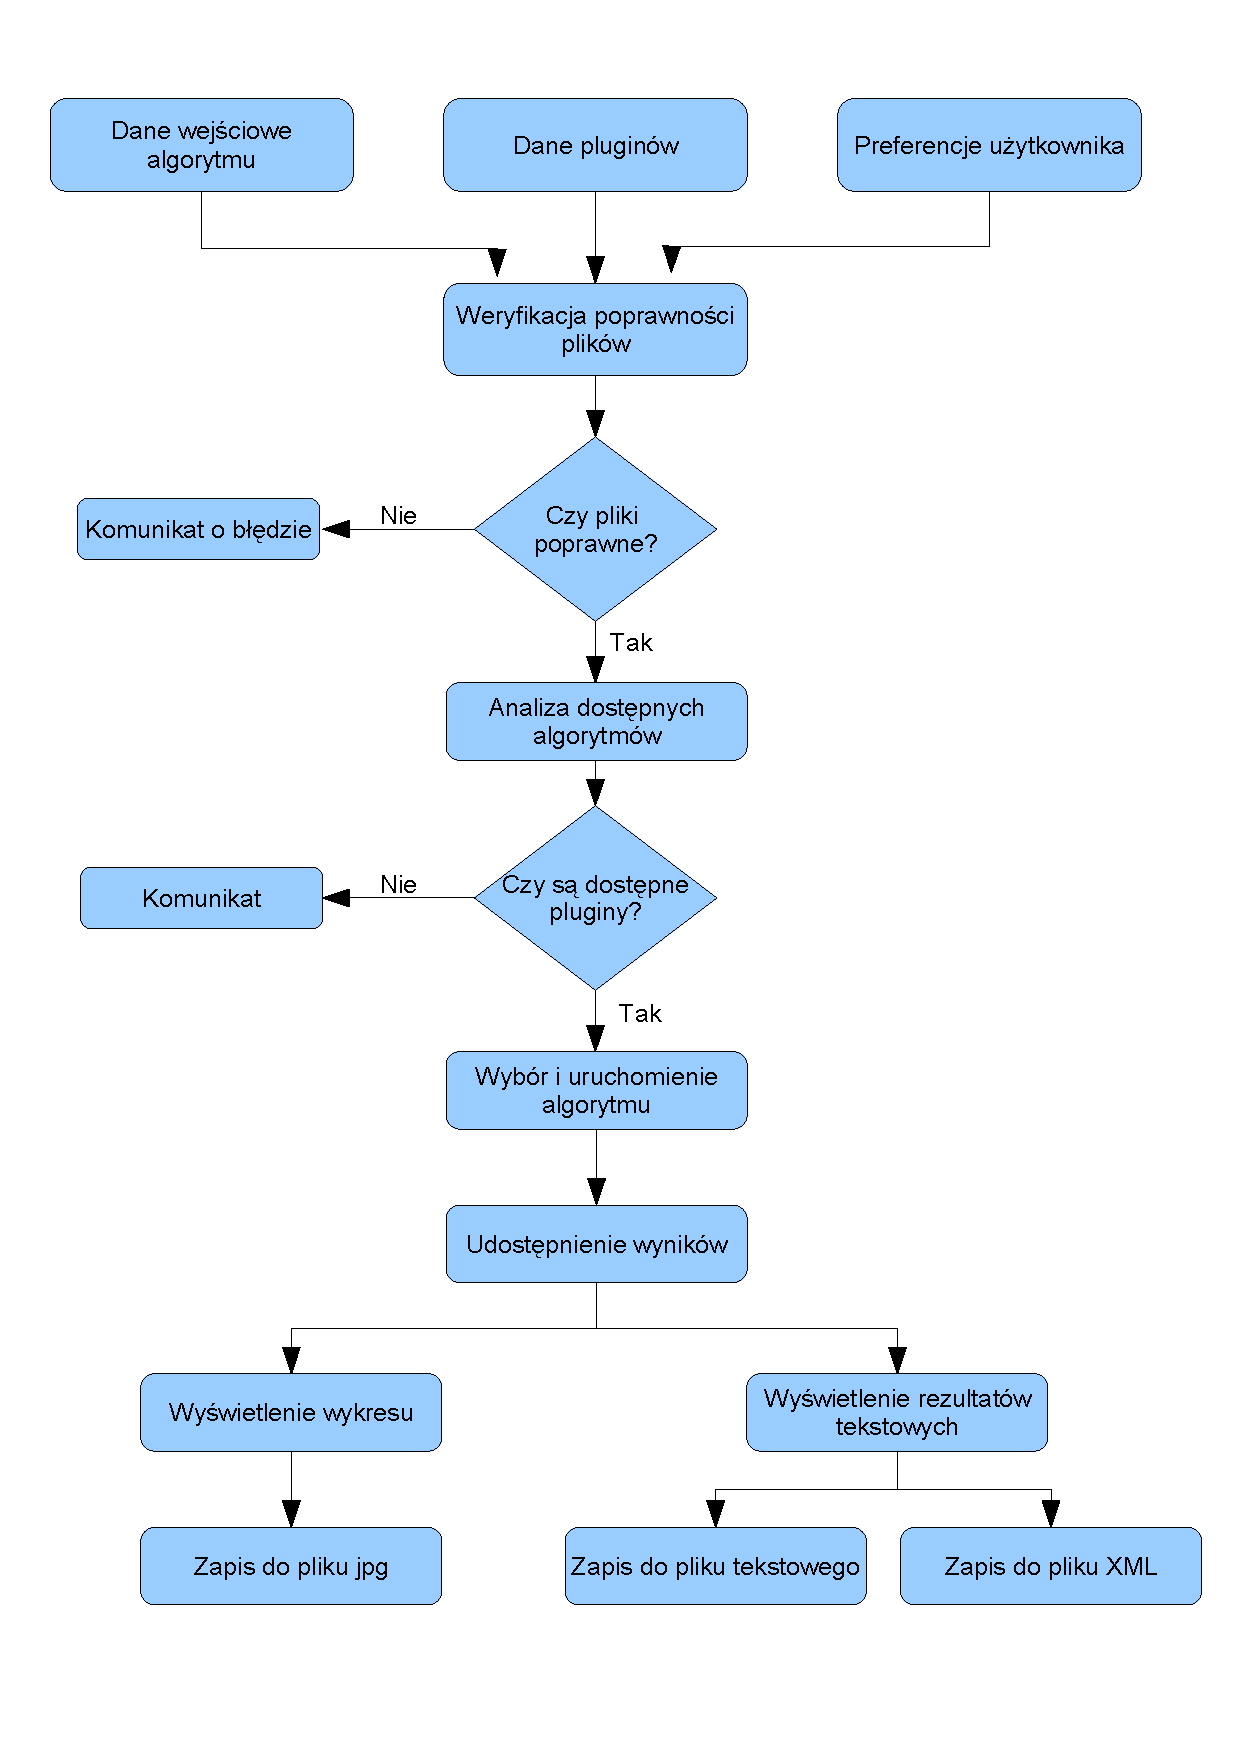
\includegraphics[scale=0.55]{figures/schemat1.pdf}
		\caption{Wykonanie algorytmu szeregowania zadań jednorodnych.}\label{rys:schemat1}
		\end{figure}
	\item Generowanie wykresu na podstawie parametrów procesorów oraz pliku XML z uszeregowaniem (podpunkt~\vref{path2}), rys.~\vref{rys:schemat2}.
		\begin{figure}[p]
        \centering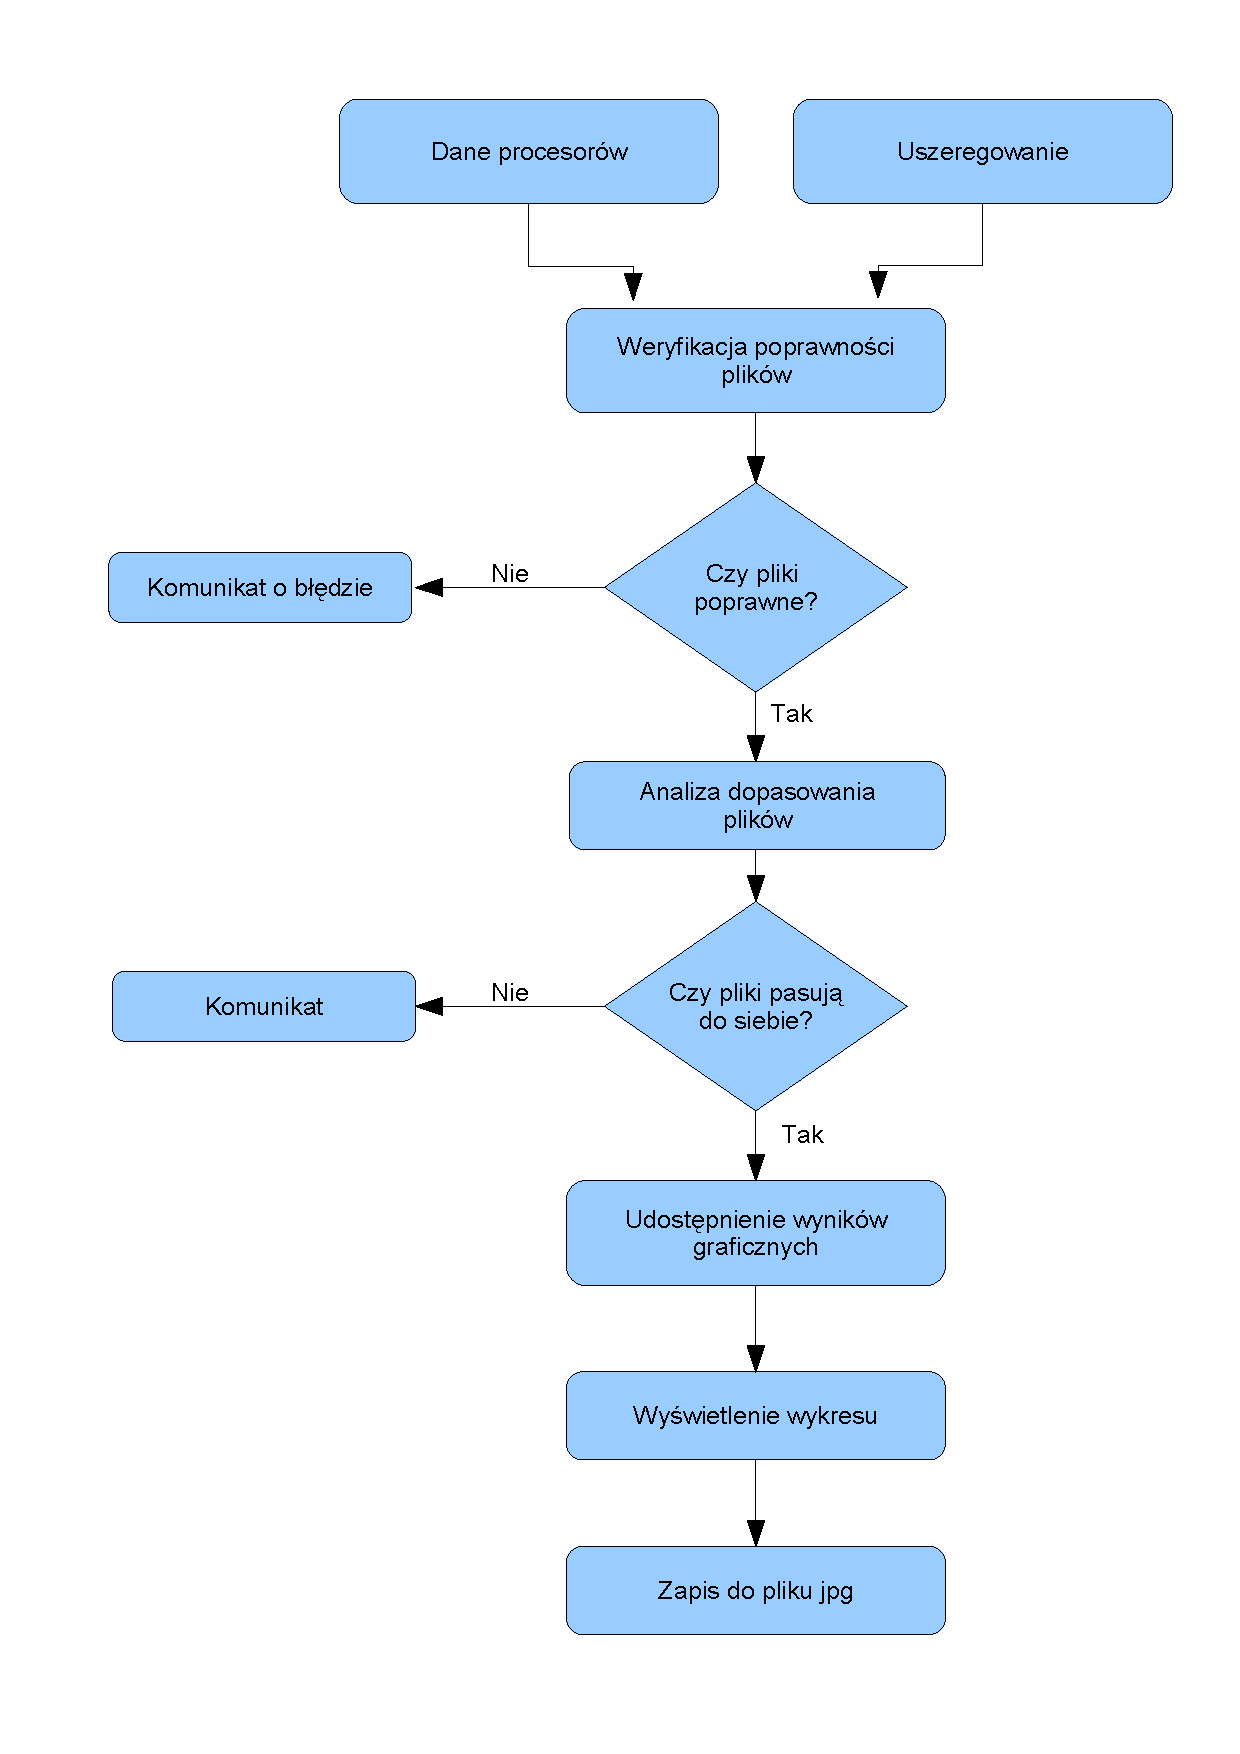
\includegraphics[scale=0.55]{figures/schemat2.pdf}
		\caption{Generowanie wykresu na podstawie gotowego uszeregowania oraz parametrów procesorów.}\label{rys:schemat2}
		\end{figure}
\end{itemize}
\afterpage{\clearpage}

\section{Wieloplatformowość}

Jak wspomniano w opisie środowiska Qt (por.~rozdział~\ref{qt}), zapewnia ono tworzenie aplikacji działających na różnych platformach programowych. Również 
program MultiSched 
można kompilować i uruchamiać zarówno pod systemem operacyjnym Windows jak i Linux. Dzięki przenośności kodu użytkownik może korzystać z aplikacji 
 w obu wymienionych środowiskach. Uniwersalność biblioteki klas Qt zapewnia poprawne działanie systemu. Interfejs programu MultiSched uruchamianego 
pod każdym systemem operacyjnym wygląda podobnie jak inne uruchamiane tam aplikacje okienkowe.

\section{Uogólniony format danych}\label{pliki}

Istotną częścią pracy było zaprojektowanie uniwersalnych formatów dla danych wejściowych oraz wyjściowych systemu. Ze względu na opisaną wcześniej 
funkcjonalność do reprezentacji tych danych został wybrany język XML. Aby ułatwić zarządzanie danymi w programie, zostały one rozdzielone na kilka 
plików. Każdy z nich jest wczytywany, parsowany i przetwarzany niezależnie, a dopiero później w zależności od wybranych funkcji odpowiednie 
wartości przekazywane są dalej.

W systemie wyróżniono następujące pliki wejściowe:
\begin{enumerate}[a)]
	\item Dane, które należy podać przy uruchamianiu algorytmu rozwiązującego problem szeregowania. Plik ten zawiera informacje takie jak:
	\begin{itemize}
		\item rozmiar wolumenu danych ($V$),
		\item liczba procesorów przetwarzających dostępnych w systemie,
		\item liczba zadań do wykonania,
		\item liczba paczek do przetworzenia,
		\item dane szczegółowe procesorów -- wymienione wcześniej w rozdziale \vref{model_przetwarzania} 
		wartości, a także koszt użycia każdego procesora,
		\item wartości niezbędne do znalezienia uszeregowania za pomocą algorytmu genetycznego; są one opcjonalne, jeśli użytkownik 
		nie zamierza wykorzystać algorytmu genetycznego, nie musi umieszczać tych danych w pliku:
		\begin{itemize}
			\item liczebność populacji,
			\item minimalna oraz maksymalna długość osobnika w populacji,
			\item liczba iteracji, po których algorytm się zatrzyma,
			\item liczba iteracji bez poprawy, po których algorytm się zatrzyma,
			\item prawdopodobieństwo krzyżowania i prawdopodobieństwo mutacji,
			\item metoda generacji populacji startowej,
			\item metoda wyboru osobników będących podstawą do stworzenia kolejnej populacji (turniejowa lub ruletka),
			\item liczebność grupy turniejowej (jeśli została wybrana metoda turniejowa),
			\item metoda wyboru punktu krzyżowania,
			\item metoda mutacji.
		\end{itemize}
	\end{itemize}
Przykładowy plik XML z danymi wejściowymi przedstawiono na listingu~\vref{lst1}.

	\item Plik opisujący wtyczki z algorytmami szeregowania, jakie będą dostępne w systemie. Zawiera następujące dane:
	\begin{itemize}
		\item nazwa algorytmu,
		\item autor algorytmu,
		\item opis,
		\item typ algorytmu (dokładny lub heurystyka) oraz ewentualnie podtyp (np.~genetyczny lub inny),
		\item informacja o tym czy algorytm uwzględnia zwracanie wyników oraz ograniczenia pamięciowe procesorów,
		\item lokalizacja wtyczki (ścieżka do biblioteki łączonej dynamicznie).
	\end{itemize}
    Przykład pliku XML z danymi wtyczki algorytmu przedstawiono na listingu~\vref{lst2}.
    
	\item Plik zawierający preferencje użytkownika dotyczące wyboru algorytmu szeregowania (typ algorytmu oraz ewentualnie podtyp),
    zob.~listing~\vref{lst3}.
\end{enumerate}

\bigskip%
Wyniki algorytmu szeregowania zadań jednorodnych mogą być również zapisane do pliku XML. Najwygodniejszym sposobem opisu uszeregowania 
okazało się przedstawienie go w postaci kolejnych akcji, z których każda opisuje przesyłanie bądź odebranie danej paczki od konkretnego procesora 
przetwarzającego. Informacje zawarte w pliku opisują:
\begin{itemize}
	\item identyfikator paczki danych,
	\item rozmiar paczki,
	\item procesor przetwarzający opisywaną paczkę,
	\item kierunek przesyłania (nadanie lub odbiór).
\end{itemize}

Dla każdego z wymienionych formatów plików został zdefiniowany dokument XML Schema opisujący strukturę i typy danych zawartych w tych plikach. 
Dokumenty te są zamieszczone w dodatku \vref{schema}.

\clearpage
\begin{listing}
\caption{Plik z danymi wejściowymi do algorytmu szeregowania zadań jednorodnych.}\label{lst1}
\begin{codeblock}
<?xml version="1.0" encoding="utf-8" ?> 
<schedule>
<dataVolumeSize>100</dataVolumeSize>
<numberOfProcessors>5</numberOfProcessors>
<numberOfPacks>10</numberOfPacks>
<numberOfTasks>1</numberOfTasks>
<processorsData>
<processor id="1">
<cost>0</cost>
<processingRate>0.980000</processingRate>
<communicationRate>0.880000</communicationRate>
<communicationStartupTime>0.370000</communicationStartupTime>
<bufferSize>0</bufferSize>			
</processor>
<processor id="2">
<cost>0</cost>
<processingRate>0.520000</processingRate>
<communicationRate>0.080000</communicationRate>
<communicationStartupTime>0.240000</communicationStartupTime>
<bufferSize>0</bufferSize>			
</processor>
<processor id="3">
<cost>0</cost>
<processingRate>0.180000</processingRate>
<communicationRate>0.910000</communicationRate>
<communicationStartupTime>0.390000</communicationStartupTime>
<bufferSize>0</bufferSize>			
</processor>
<processor id="4">
<cost>0</cost>
<processingRate>0.370000</processingRate>
<communicationRate>0.590000</communicationRate>
<communicationStartupTime>0.880000</communicationStartupTime>
<bufferSize>0</bufferSize>			
</processor>
<processor id="5">
<cost>0</cost>
<processingRate>0.780000</processingRate>
<communicationRate>0.500000</communicationRate>
<communicationStartupTime>0.230000</communicationStartupTime>
<bufferSize>0</bufferSize>			
</processor>
</processorsData>
<geneticAlgorithmParameters>
<populationSize>10</populationSize>	
<maxLengthOfIndividualsInStartPopulation>
15
</maxLengthOfIndividualsInStartPopulation>
<mutationPercent>0.1</mutationPercent>
<crossPercent>30</crossPercent>
<numberOfIterationsToStop>500</numberOfIterationsToStop>
<numberOfIterationsWithoutImprovementToStop>
30
</numberOfIterationsWithoutImprovementToStop>
<tournamentGroupSize>0</tournamentGroupSize>
<startPopulationGenerationMethod>
0
</startPopulationGenerationMethod>
<minLengthOfIndividualsInStartPopulation>
0
</minLengthOfIndividualsInStartPopulation>
<selectionMethod>2</selectionMethod>
<methodOfChoosingCrossPoint>2</methodOfChoosingCrossPoint>
<methodOfMutation>2</methodOfMutation>
</geneticAlgorithmParameters>
</schedule>
\end{codeblock}
\end{listing}

\clearpage
\begin{listing}
\caption{Plik z opisem wtyczek implementujących algorytmy szeregowania zadań jednorodnych.}\label{lst2}
\begin{codeblock}
<?xml version="1.0" encoding="utf-8" ?> 
<plugins>
<plugin>
<algorithm>
<author>Joanna Zietkiewicz</author>
<name>Branch and Bound</name>
<description>Algorytm dokladny dla wieloetapowego problemu 
szeregowania zadan jednorodnych</description>
<type>exact</type>
<returnResults>true</returnResults>
<bufferConstraints>false</bufferConstraints>
</algorithm>
<location>plugins/zietkiewicz.dll</location>
</plugin>
<plugin>
<algorithm>
<author>Przemyslaw Daniel</author>
<name>Branch and Bound</name>
<description>Algorytm dokladny szeregowania zadan jednorodnych 
w heterogenicznym systemie komputerowym</description>
<type>exact</type>
<returnResults>false</returnResults>
<bufferConstraints>false</bufferConstraints>
</algorithm>
<location>plugins/daniel.dll</location>
</plugin>
<plugin>
<algorithm>
<author>Pawel Rogala</author>
<name>Algorytm genetyczny</name>
<description>Algorytm genetyczny dla problemu dystrybucji 
obliczen w rozproszonym systemie komputerowym</description>
<type>heuristic</type>
<subtype>genetic</subtype>
<returnResults>false</returnResults>
<bufferConstraints>false</bufferConstraints>
</algorithm>
<location>plugins/rogala.dll</location>
</plugin>
</plugins>
\end{codeblock}
\end{listing}

\begin{listing}
\caption{Plik zawierający preferencje użytkownika dotyczące wyboru algorytmu szeregowania zadań jednorodnych.}\label{lst3}
\begin{codeblock}
<?xml version="1.0" encoding="utf-8" ?> 
<preferences>
<type>heuristic</type>
<subtype>genetic</subtype>
</preferences>
\end{codeblock}
\end{listing}



\chapter{Implementacja}

\section{Wykorzystane technologie i narzędzia}

Bieżący rozdział opisuje język programowania, narzędzia oraz technologie, jakie zostały użyte przy realizacji pracy magisterskiej. Na szczególną 
uwagę zasługuje opis środowiska programistycznego Qt udostępniającego szeroki wachlarz narzędzi i funkcji, dla wielu różnych platform komputerowych.

\subsection{Język programowania}

Jako język programowania, w którym został stworzony opisany system, wybrano C++. Na decyzję wpłynął fakt, że dostępne programy implementujące 
algorytmy szeregowania zadań jednorodnych były napisane w tym właśnie języku.
C++ powstał w latach osiemdziesiątych XX wieku. Język ten łączy w sobie dwa elementy -- składnię C (dzięki temu jest kompatybilny z aplikacjami 
napisanymi w tym języku) oraz możliwość programowania obiektowego. 

\definicja{Programowanie obiektowe} (\akronim{OOP}, \english{object-oriented programming}) to metodologia tworzenia programów, która definiuje je za pomocą obiektów 
pogrupowanych w klasy. Są to elementy łączące stan rzeczywistości (czyli dane) i zachowanie (czyli metody). Obiekty te komunikują się ze sobą 
w celu wykonywania pewnych zadań. Celem tego jest ułatwienie konserwacji, wykorzystanie fragmentów kodu w wielu aplikacjach oraz samo 
pisanie i zrozumienie kodu. Programowanie obiektowe jest bardzo intuicyjne i zbliżone do natury postrzegania świata przez człowieka. 
Mózg człowieka naturalnie klasyfikuje rzeczywiste obiekty w grupy, zwracając przy tym uwagę na wspólne cechy i zachowania. Dzięki tej 
właściwości w programowaniu jego twórca jest w stanie panować nad większymi strukturami, które lepiej i prościej modelują rzeczywistość.

Główne cechy programowania obiektowego to:
\begin{itemize}
	\item \textbf{Enkapsulacja} -- ukrywanie implementacji. Oznacza to, że stan obiektu może być zmieniany tylko przez jego wewnętrzne metody. 
	Każdy obiekt udostępnia innym metody do komunikacji, co nazywamy interfejsem.
	\item \textbf{Polimorfizm} -- referencje i kolekcje obiektów mogą dotyczyć obiektów różnego typu, a wywołanie metody dla referencji spowoduje 
	zachowanie odpowiednie dla pełnego typu obiektu wywoływanego.
	\item \textbf{Dziedziczenie} -- umożliwia definiowanie i tworzenie specjalizowanych obiektów na podstawie bardziej ogólnych. Tak więc dla 
	specjalizowanych obiektów nie zachodzi potrzeba definiowania całej funkcjonalności, a jedynie tej, której nie posiada obiekt ogólniejszy.
\end{itemize}

\subsection{Biblioteka Qt}\label{qt}

Qt (\cite{qt}) jest wieloplatformowym środowiskiem służącym do programowania \akronim{GUI} (\english{Graphical User Interface}) 
w języku C++. Produkt ten jest rozwijany przez firmę Trolltech (\cite{trolltech}). Obecnie w użyciu są wersje dostępne dla 
następujących platform:  Windows, X11 (Linux, BSD, Solaris), Mac OS X, a także dla tzw. urządzeń wbudowanych opartych na systemach linuksowych. 
Dzięki różnorodności licencji użytkownika, na których dostępna jest ta platforma, stała się ona podstawą wielu udanych przedsięwzięć programistycznych. 
W roku 1996 roku została wprowadzona na rynek komercyjna wersja środowiska, oprócz tego dostępna jest także wersja otwarta (\english{open source}) oraz 
dla specjalnych celów również akademicka i edukacyjna. Godna uwagi jest tu właśnie wersja otwarta. Jej istotną cechą jest brak kosztów użytkowania, 
dzięki czemu produkt staje się dostępny praktycznie dla każdego programisty. Edycja ta jest udostępniana na licencji \akronim{GPL} (\english{General Public 
License}), dlatego też należy pamiętać, że produkty stworzone za jej pomocą, muszą być udostępniane również zgodnie z zasadami tej licencji. 
Wersja open source była dostępna początkowo tylko dla systemów linuksowych (od 2000 roku), jednak w roku 2004 firma Trolltech wydała również 
edycję dla platformy Mac OS X, a w 2005 także dla Windows. Windowsowa edycja produktu korzysta z darmowego kompilatora MinGW, więc w związku 
z tym nie wymaga posiadania narzędzi takich, jak np.~MS Visual C++, które to są używane przez komercyjne wydanie Qt. W obecnej chwili 
na rynku dostępna jest (dla wszystkich wymienionych wcześniej platform) wersja 4.1.2. Pracę z Qt wspomaga narzędzie qmake, które służy do organizowania 
kompilacji na różnych platformach i kompilatorach.

O popularności produktu Qt świadczy między innymi fakt, że jest on podstawą znanego uniksowego środowiska graficznego KDE (na razie ciągle jeszcze 
trzecia edycja biblioteki), a także popularnej przeglądarki internetowej Opera.

Qt stanowi obszerne środowisko programistyczne składające się z wielu modułów. Dzięki temu programista zostaje wyposażony w całą niezbędną do budowy interfejsów 
funkcjonalność. Środowisko cechuje się dużą intuicyjnością, a doskonale napisana dokumentacja pozwala programiście szybko przyswoić sobie 
zasady jego funkcjonowania i współpracy z pakietem.

Centralną część środowiska Qt stanowi \akronim{MOC} (\english{Meta Object Compiler}). Jego zadaniem jest obsługa wszystkich rozszerzeń C++, które są 
dostarczane przez Qt. Podczas kompilacji wykonywany jest proces mający na celu przekształcenie kodu opartego na Qt na dający się skompilować 
na danej platformie. Dzięki temu zapewniona zostaje przenośność aplikacji.

\subsubsection*{Składniki platformy Qt}

Platforma programistyczna Qt obejmuje następujące składniki:
\begin{enumerate}[a)]
	\item \textbf{Qt Assistant} -- to w pełni dostosowana do wymagań użytkownika przeglądarka dokumentacji oraz plików pomocy. Jej działanie jest 
	zbliżone do przeglądarki internetowej. Dokumentacja jest prezentowana jako zbiór hiperłączy, a zawartość plików może być wyświetlana 
	zarówno jako tekst jak i HTML. Dzięki temu użytkownik w łatwy sposób może dotrzeć do opisów wybranych metod, a także przykładów. Assistant 
	udostępnia funkcję wyszukiwania informacji oraz tworzenie grup ,,ulubionych'' dla preferowanych stron. Dużą zaletą jest możliwość wyświetlenia 
	każdej strony w kolejnej zakładce. Przeglądarka ta może również stanowić podstawę do zbudowania systemu pomocy dla konkretnej aplikacji 
	stworzonej za pomocą platformy Qt. Uruchomiona aplikacja Assistant przedstawiona jest na rys.~\vref{rys:assistant}.
	\begin{figure}[ht]
	\centering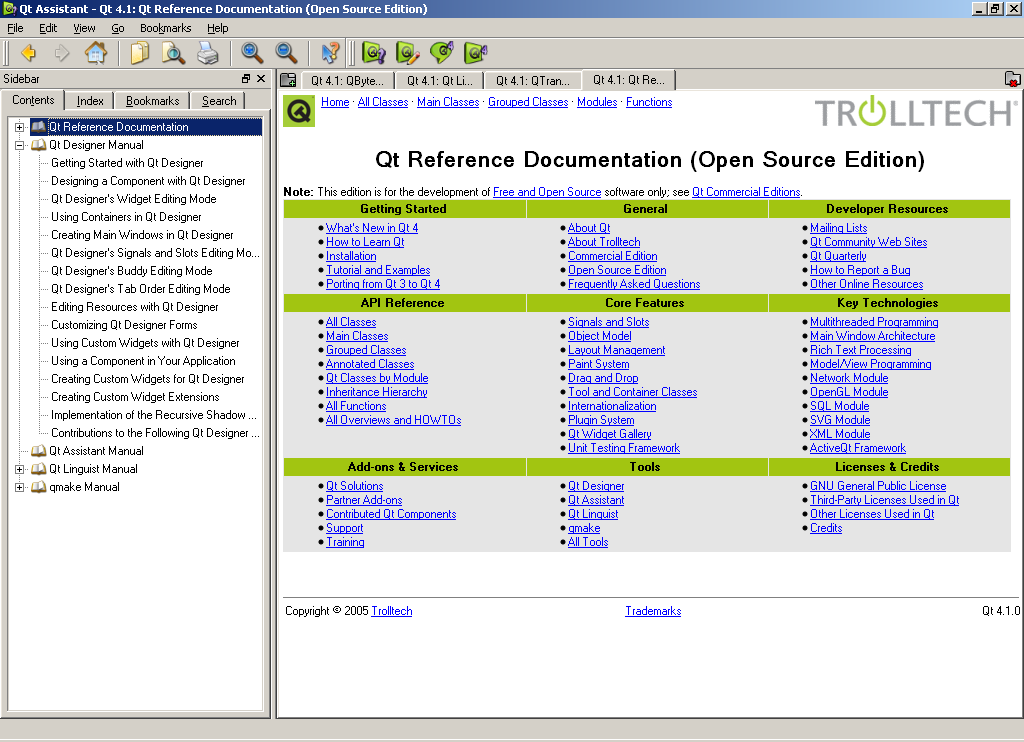
\includegraphics[scale=0.4]{figures/assistant.png}
	\caption{Qt Assistant.}\label{rys:assistant}
	\end{figure}

	\item \textbf{Qt Designer} -- jest bardzo funkcjonalnym narzędziem wspomagającym budowę interfejsów użytkownika. Umożliwia szybkie tworzenie i rozwój 
	GUI aplikacji. Dzięki podejściu \definicja{przeciągnij i upuść} (\english{drag-and-drop}) twórca interfejsu może go zaprojektować precyzyjnie. 
	Qt Designer zawiera takie funkcje jak: możliwość podglądu, automatyczne rozmieszczenie kontrolek, wsparcie dla tworzenia własnych kontrolek oraz 
	zaawansowany edytor właściwości. Interfejs stworzony w Qt wygląda identycznie jak w przypadku innych aplikacji uruchamianych na konkretnej 
	platformie. Wsparcie projektowania interfejsu zapewnia \akronim{UIC} (\english{User Interface Compiler}). Jest on prawie zawsze wywoływany przez 
	program \texttt{make}. Jego celem jest wygenerowanie plików nagłówkowych i źródeł na podstawie stworzonych za pomocą Designera plików \texttt{.ui}, które 
	opisują interfejs. Pliki \texttt{.ui} są w istocie plikami zapisanymi w języku XML a UIC stanowi interpreter przekształcający je w w pliki 
	\texttt{.h} i \texttt{.cpp}. Przykładowe tworzenie interfejsu za pomocą designera przedstawione jest na rys.~\vref{rys:designer}
	\begin{figure}[p]
	\centering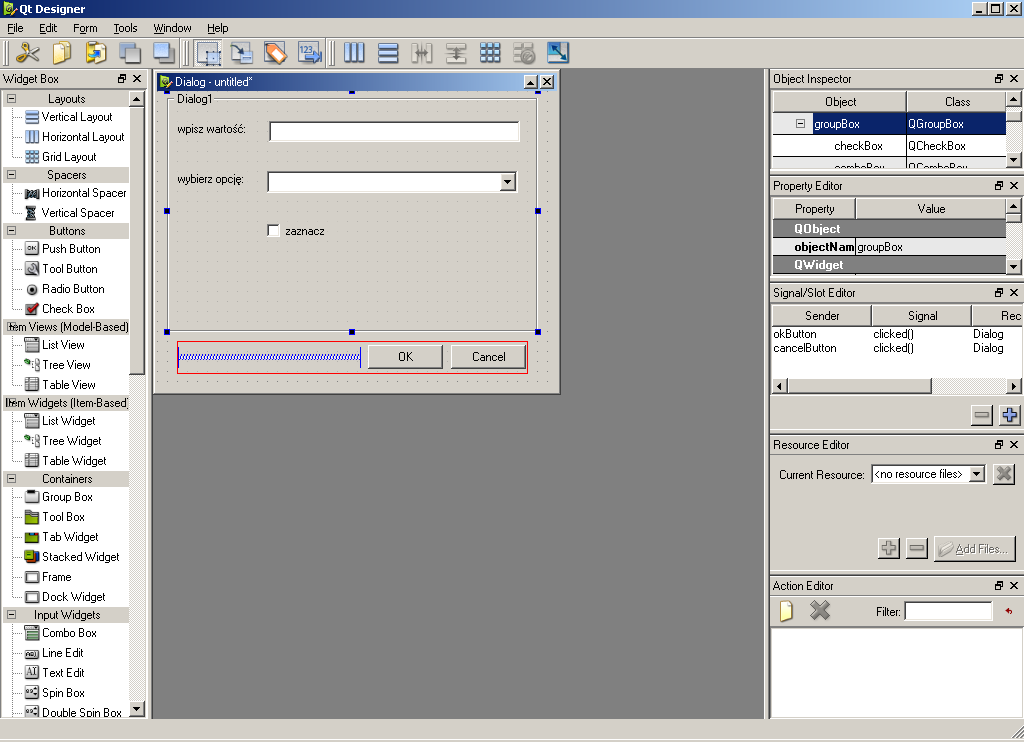
\includegraphics[scale=0.4]{figures/designer.png}
	\caption{Qt Designer.}\label{rys:designer}
	\end{figure}
	
	\item \textbf{Qt Linguist} -- stanowi zbiór narzędzi przeznaczonych do internacjonalizacji aplikacji. Moduł ten dostarcza interfejs skracający i wspomagający 
	proces tłumaczenia interfejsu użytkownika na język używany w systemie operacyjnym. Umożliwia zebranie wszystkich tekstów, opisów i komunikatów, 
	jakie są prezentowane użytkownikowi i pozwala łatwo zarządzać nimi oraz ich tłumaczeniami na języki obsługiwane przez program. Poprzez zastosowanie 
	dwukierunkowych algorytmów pisania wspierających Unicode, Qt pozwala nawet na zastosowanie takich języków jak hebrajski lub arabski. Wykorzystanie Qt Linguist 
	przedstawia rys.~\vref{rys:linguist}.
	\begin{figure}[p]
	\centering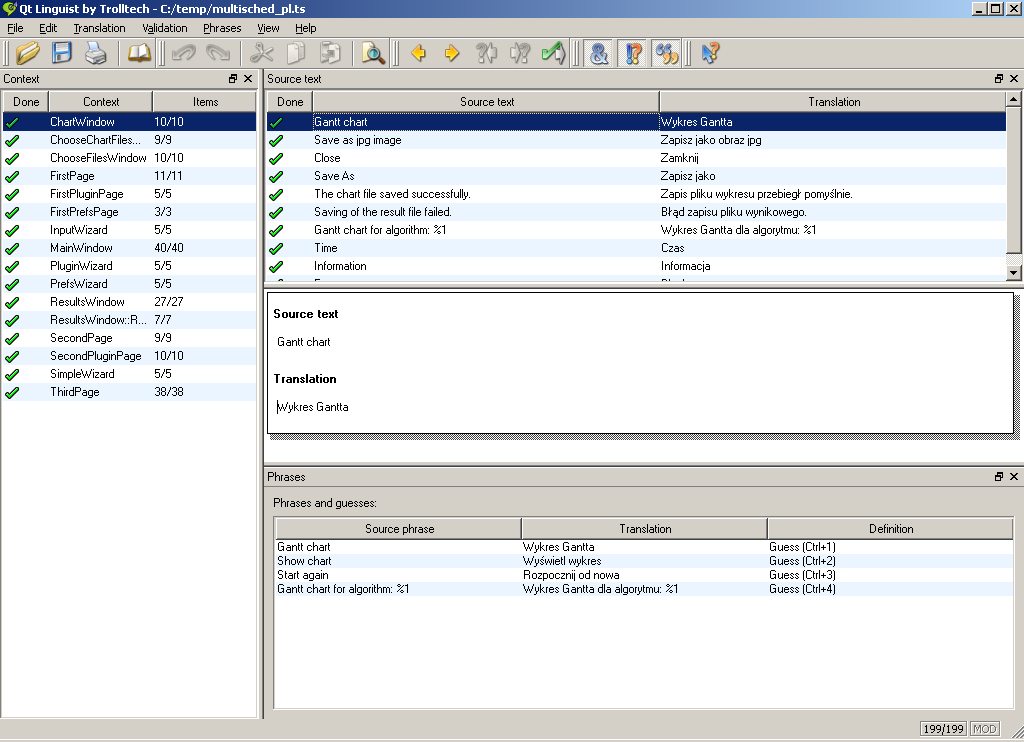
\includegraphics[scale=0.4]{figures/linguist.png}
	\caption{Qt Linguist.}\label{rys:linguist}
	\end{figure}
    \afterpage{\clearpage}

	\item \textbf{Biblioteka klas Qt} -- najważniejsza część całego środowiska programistycznego. Implementuje ona ponad 400 klas składających się 
	na API Qt. Klasy te służą nie tylko do tworzenia i obsługi interfejsu użytkownika, ale udostępniają również szereg innych przydatnych 
	funkcjonalności. Wiele z nich stanowi wypełnienie luk w standardowych bibliotekach C++ i dostarcza ,,brakujących'' tam funkcji. API Qt jest 
	w pełni dojrzałym modelem obiektowym, pozwala na obsługę baz danych, sieci komputerowych, języka XML, a nawet zapewnia integrację z OpenGL.	
\end{enumerate}

\subsubsection*{Mechanizm sygnałów i slotów}

Istotnym elementem środowiska Qt jest wykorzystanie innowacyjnego mechanizmu służącego do komunikacji między kontrolkami i obiektami.
Polega on na wysyłaniu odpowiedniego sygnału w momencie, gdy zachodzi jakieś zdarzenie. Sloty natomiast są funkcjami wywoływanymi jako 
odpowiedź na dany sygnał. Każdy sygnał może mieć przyporządkowanych 0, 1 lub więcej metod obsługujących go. I odwrotnie -- jeden slot 
może być odpowiedzią na wiele sygnałów. Zarządzanie sygnałami i slotami odbywa się za pomocą funkcji \code{connect} i \code{disconnect}.
Każda kontrolka ma pewną liczbę predefiniowanych sygnałów i slotów, jednak programista ma możliwość dodawania, w miarę potrzeby, własnych 
poprzez utworzenie podklasy danej kontrolki.

\subsection{Kompilator MinGW}\label{mingw}

MinGW (\english{Minimalist GNU for Windows}, \cite{mingw}) to zestaw plików nagłówkowych i bibliotek dla platformy Windows wraz z kompilatorem 
GCC (\english{GNU Compiler Collection} -- zestaw kompilatorów tworzony w ramach projektu GNU), który jest popularny w systemach linuksowych. Jak wskazuje 
nazwa tego narzędzia, MinGW zawiera minimalną wersję kompilatora GCC.

\subsection{XML}

W związku z ciągłym rozwojem technologii informatycznych wykształciło się zapotrzebowanie na uniwersalny i czytelny format opisu danych, 
którego pożądaną cechą byłaby elastyczność i rozszerzalność. Naprzeciw tym potrzebom wyszedł właśnie \akronim{XML} (\english{eXtensible Markup Language} -- 
rozszerzalny język znaczników). XML~\cite{xml} to otwarty standard, który został opracowany przez \akronim{W3C} 
(\english{World Wide Web Consortium}). Wywodzi się on z \akronim{SGML} (\english{Standard Generalized Markup Language} 
-- standaryzowany nadrzędny język znaczników) i jest uniwersalnym tekstowym formatem pozwalającym na przechowywanie danych, a także 
przesyłanie ich. XML pozwala również na tworzenie nowych języków przy pomocy znaczników układających się w strukturę hierarchicznego drzewa.

XML ma możliwość definiowania dowolnej nieograniczonej liczby własnych znaczników. Każdy z tych znaczników może zawierać pewne atrybuty. 
Nazwy nadawane są znacznikom przez użytkownika, a ich znaczenie zależy od interpretacji autora dokumentu XML. Każdy otwarty znacznik musi 
zostać zamknięty.

\begin{listing}[th]
\caption{Przykład pliku w formacie XML.}
\begin{codeblock}
<person name="Edek z Krainy Kredek">
<height unit="cm">190</height>
<weight unit="kg">75</weight>
</person>
\end{codeblock}
\end{listing}

Do opisu danych zawartych w dokumencie XML można wykorzystać DTD (\english{Document Type Definition}) lub XML Schema.
\begin{itemize}
	\item \textbf{DTD} -- pozwala na zdefiniowanie ograniczeń dotyczących struktury dokumentu. Zawiera definicje wszystkich elementów dokumentu, 
	ich atrybutów oraz dopuszczalnych wartości, jakie mogą być przyjmowane przez te elementy. DTD może być zawarte w tym samym pliku, co 
	dokument XML, częściej jednak, ze względów praktycznych, zostaje umieszczone w odrębnym pliku. Dzięki temu może zostać wykorzystane 
	jeszcze dla innych elementów.
	\item \textbf{XML Schema} -- uznawane jest za następcę DTD. Jednak w odróżnieniu od niego, XML Schema jest również dokumentem XML 
	(zgodnym z jego specyfikacją). Ma również o wiele większe możliwości, między innymi pozwala na zdefiniowanie typów danych (nie było to możliwe w DTD). 
	Pliki Schema zazwyczaj zapisuje się z rozszerzeniem \texttt{.xsd} (pochodzi ono od \emph{XML Schema Definition}).
\end{itemize}

Aby uzyskać dostęp do danych zawartych w dokumencie XML można skorzystać z parsera. Parser taki analizuje składnię i umożliwia manipulację 
danymi. Rozróżnia się dwa podstawowe typy parserów XML:
\begin{itemize}
	\item \textbf{DOM} -- \textbf{\emph{Document Object Model}} -- Dzięki hierarchicznej strukturze dokumentu XML można go łatwo przedstawić w pamięci komputera 
	za pomocą popularnych struktur danych. Na tym fakcie opiera się właśnie parser DOM. Dokonuje on wczytania całego dokumentu do drzewa obiektów. 
	Użytkownik dostaje w wyniku wskaźnik do korzenia tego drzewa. Dostęp do każdego elementu można uzyskać przeglądając je poczynając od korzenia. 
	Model ten jest bardzo wygodny, ponieważ w łatwy sposób można operować na wszystkich danych. Jednak istotną jego wadą jest duże zapotrzebowanie 
	na pamięć, w przypadku dużych dokumentów może to sprawiać problemy.
	\item \textbf{SAX} -- \textbf{\emph{Simple Api for XML}} -- Parser ten jest oparty na obsłudze zdarzeń. Dane są przetwarzane w trakcie analizy dokumentu. 
	SAX działa wywołując odpowiednie funkcje po napotkaniu na odpowiednie znaczniki (np.~reakcja na znacznik otwierający lub zamykający bądź na atrybut).
	Dzięki temu SAX działa o wiele szybciej od DOMa, nie potrzebuje wiele pamięci i jest polecany szczególnie dla dużych dokumentów.
\end{itemize}

Oprócz opisu i przechowywania danych rolą języka XML jest też ich prezentacja. Dzięki arkuszom stylów CSS oraz programowalnych arkuszy 
stylów (XSL), które zostały zaprojektowane specjalnie dla XML-a mamy możliwość różnorodnej prezentacji dokumentu w przeglądarce internetowej. 

Podsumowując, jako najistotniejsze można wymienić następujące cechy XMLa:
\begin{itemize}
	\item uniwersalność,
	\item elastyczność,
	\item łatwość przetwarzania,
	\item czytelność.
\end{itemize}

\section{Główne klasy programu}

W podrozdziale tym zostały opisane najważniejsze klasy programu MultiSched. Ze względu na dużą ich liczbę do opisu wybrane zostały tylko te, 
które zawierają metody sterujące programem. Opis ten nie uwzględnia klas prostych, czyli przechowujących jedynie dane, a także klas 
reprezentujących pomniejsze okna dialogowe.

\subsection{MainWindow}

Klasa ta reprezentuje główne okno interfejsu graficznego programu. Odpowiada ona w zasadzie za całe sterowanie programem. Z poziomu tej 
klasy tworzone są obiekty klas opisanych poniżej, a na nich następnie wywoływane odpowiednie metody. MainWindow poprzez menu daje dostęp do wszystkich funkcji 
systemu, jakie mógłby wywołać użytkownik. Na największą uwagę zasługuje metoda \code{schedule()}. Jej zadaniem jest sprawdzenie, czy wybrana przez 
użytkownika wtyczka z algorytmem szeregującym zadania jest zgodna z interfejsem \code{PluginInterface}. Jeśli tak, to przygotowywany jest obiekt 
z danymi wejściowymi do algorytmu a następnie wywoływana funkcja \code{findSchedule(ScheduleData *data, AlgorithmResults* results)}. 
Po jej wykonaniu użytkownik dostaje informację o wynikach wywoływanego algorytmu szeregowania zadań jednorodnych.

\subsection{Reader}

Klasa \code{Reader} jest odpowiedzialna za wczytywanie wszelkich danych do programu (podanych w postaci plików XML). Kolejnym jej zadaniem jest 
parsowanie danych oraz stworzenie z nich odpowiednich obiektów typu bean. Metody parsujące wykorzystują jeden z opisanych wyżej parserów XMLa (DOM). 
Dostępna w bibliotece Qt klasa \code{QDomNode} oraz jej podklasy umożliwiają operowanie na dokumencie XML traktowanym jako drzewo elementów. 
Kolejnym krokiem po przetransformowaniu dokumentu XML do postaci obiektu zawierającego zbiór danych jest ich weryfikacja. Funkcje walidujące 
sprawdzają zgodność każdej odczytanej z pliku wartości z zasadami poprawności opisanymi w dokumentach XML Schema.

\subsection{DecisionMaker}

Na podstawie preferencji użytkownika oraz informacji zawartych w plikach wejściowych podejmowana jest decyzja dotycząca algorytmów możliwych 
do uruchomienia dla wczytanych danych. Za decyzję tę odpowiada metoda \code{makeDecision()}. Jej rezultatem jest lista indeksów wtyczek, które 
użytkownik będzie mógł uruchomić.

\subsection{ResultsWindow}

Klasa ta jest reprezentacją okna wyświetlającego wyniki uszeregowania. W oknie głównym prezentowane są wyniki tekstowe działania algorytmu. 
Zawiera ona również metody odpowiadające za zapis rezultatów do plików - XML oraz w formacie tekstowym. 

\subsection{ChartWindow}

Za okno wyświetlania graficznych wyników uszeregowania jest odpowiedzialna klasa \code{ChartWindow}. Przy pomocy obiektów klas \code{QImage}, 
\code{QPainter}, \code{QPen} oraz \code{QBrush} w oknie tym rysowany jest wykres Gantta ilustrujący przesyłanie paczek danych do i 
z procesorów oraz ich przetwarzanie. Tworzeniem wykresu zajmują się dwie metody:
\begin{itemize}
	\item \code{findImageSize()} -- znajduje rozmiar tworzonego obrazka. Wymiary te są obliczane na podstawie danych o kolejnych akcjach (czyli wysyłaniu 
	lub odbieraniu paczek) oraz informacji o parametrach procesorów. Minimalny rozmiar wykresu dopasowany jest do wymiarów całego okna. W przypadku, 
	gdy wykres zajmuje więcej miejsca, początkowy rozmiar okna jest taki sam, jednak istnieje możliwość przeglądania rysunku przy użyciu pasków 
	przewijania.
	\item \code{paintChart()} -- metoda odpowiadająca za narysowanie wykresu na obiekcie klasy \code{QImage}. Podobnie jak funkcja opisana powyżej, ta również 
	wykorzystuje parametry procesorów i łącz oraz dane uszeregowania. W celu uczynienia wykresu bardziej czytelnym, kolejnym procesorom zostały 
	przyporządkowane różne kolory. Całkowita liczba kolorów wynosi 10, więc w przypadku większej liczby maszyn, będą one przydzielane na zasadzie dzielenia 
	ich numerów modulo 10. Aby odróżnić wysyłanie paczek od ich odbierania, akcje te są zaznaczone na wykresie tym samym kolorem ale różną 
	fakturą pędzla.
\end{itemize}

\medskip
Metoda \textbf{\emph{save()}} zajmuje się zapisem gotowego wykresu do pliku w formacie JPG.

\subsection{XmlWriter}

Klasa \code{XmlWriter} zawiera metody odpowiedzialne za zapis danych do plików w formacie XML. Zaimplementowane są w niej 4 funkcje:
\begin{itemize}
	\item \code{writeInputFile(QString filePath, ScheduleData *data)} -- funkcja wykorzystywana przez kreator pliku wejściowego. Zapisuje ogólne informacje 
	wejściowe, dane łącz, procesorów i ewentualnie parametry algorytmu genetycznego podane przez użytkownika do postaci XMLa.
	\item \code{writePluginsFile(QString filePath, QList $<$PluginData*$>$ plugins)} -- funkcja wykorzystywana przez kreator pliku z informacją o dostępnych 
	algorytmach.
	\item \code{writePrefsFile(QString filePath, int prefs, int prefsDetails)} -- zapis preferencji użytkownika dotyczących wyboru algorytmu 
	znajdującego uszeregowanie.
	\item \code{writeXmlToFile(QString filePath, AlgorithmResults *algorithmResults)} -- zapis obliczonego uszeregowania w postaci zbioru akcji.
\end{itemize}

\subsection{PluginInterface}

Klasa ta jest interfejsem, który musi być zaimplementowany przez każdą klasę kompilowaną do biblioteki łączonej dynamicznie stanowiącej wtyczkę 
z algorytmem szeregowania zadań jednorodnych. \code{PluginInterface} zawiera jedną wirtualną metodę \code{findSchedule(ScheduleData *data, 
AlgorithmResults* results)}. Każda wtyczka zawiera własną implementację tej metody, warunkiem jest tylko, aby znajdowała ona uszeregowanie, 
a wynik zapisywała do obiektu \code{results}, do którego wskaźnik jest podawany jako parametr do funkcji.

\section{Prezentacja wyników}

Ważną częścią wymaganej funkcjonalności systemu jest prezentacja wyników otrzymanych po wykonaniu wybranego algorytmu. W zależności od potrzeb 
użytkownik aplikacji może skorzystać z opcji prezentacji wyników w postaci tekstowej lub graficznej.

\subsection{Wyniki tekstowe}

Najważniejszym elementem prezentacji wyników algorytmu szeregowania zadań jednorodnych w postaci tekstowej jest podanie znalezionego przydziału 
poszczególnych części zadań do procesorów oraz ich rozmiaru. Paczki danych są wymienione w kolejności ich przesyłania, przy każdej transmisji 
jest zaznaczone czy stanowi ona dostarczenie części do procesora, czy też odbiór.

Wynikiem działania każdej z zaimplementowanych wtyczek jest też długość znalezionego uszeregowania czyli $C_{max}$.

Oprócz wyżej wymienionych rezultatów każda wtyczka może udostępnić np.~wyniki pośrednie działania algorytmu. Tak jest w przypadku algorytmu 
genetycznego -- użytkownik po wybraniu opcji prezentacji wyników tekstowych ma dostęp do takich danych jak numer populacji, liczba krzyżowań i 
mutacji, liczba osobników oraz genów w chromosomach, itp.

\subsection{Wykres}

Graficzną prezentację wyników działania algorytmu stanowi wykres Gantta ilustrujący znalezione uszeregowanie. Przedstawia on przydział wszystkich 
paczek do procesorów oraz ich transmisję. Oś pozioma wykresu pokazuje upływ czasu. Czerwonym kolorem na tej osi została zaznaczona długość 
znalezionego uszeregowania ($C_{max}$). Wszystkie paczki przydzielone do danego procesora są wyróżnione poprzez zaznaczenie tym samym kolorem. 
Kolor dla każdego procesora jest przyporządkowany na zasadzie numeru procesora modulo 10. Na osi pionowej najwyżej znajduje się zawsze procesor 
nadzorca a dopiero poniżej procesory przetwarzające. Dla inicjatora wykres pokazuje czas przesyłania danych do procesora przetwarzającego, 
natomiast dla procesorów przetwarzających ilustruje czas przetwarzania paczki danych.

\section{Interfejs użytkownika}

\subsection{Ogólne informacje}
System do oceny i porównywania algorytmów szeregowania zadań jednorodnych jest wyposażony w interfejs graficzny. Interfejs ten zapewnia 
dostęp do wszystkich funkcji, jakie oferuje program. Wszystkie elementy interfejsu zostały stworzone w oparciu o komponenty dostarczone przez 
środowisko Qt. Kontrolki na formularzach są rozmieszczone za pomocą tzw. layoutów. Najczęściej wykorzystane w aplikacji ułożenia komponentów to: 
\code{QGridLayout}, \code{QHBoxLayout}, \code{QVBoxLayout} oraz \code{BorderLayout}. Ten ostatni nie jest standardową klasą biblioteki Qt, 
natomiast został zaimplementowany 
w jednym z przykładów. Użyto go w programie ze względu na wygodę sposobu rozmieszczania kontrolek (opartego na stronach świata). Poszczególne elementy 
można umieszczać w następujących miejscach kontrolki-rodzica:
\begin{itemize}
	\item \textbf{North} -- północ,
	\item \textbf{South} -- południe,
	\item \textbf{East} -- wschód,
	\item \textbf{West} -- zachód,
	\item \textbf{Center} -- centrum.
\end{itemize}

Rozmiar wszystkich okien w programie może być zmieniany przez użytkownika.

Interfejs użytkownika jest dostępny w dwóch wersjach językowych -- angielskiej i polskiej. Do realizacji wielojęzyczności zostało 
wykorzystane opisane wcześniej narzędzie Qt Linguist. Domyślnie program uruchamiany jest z interfejsem angielskim. Opcja zmiany języka 
interfejsu jest umieszczona w menu programu, można z niej korzystać podczas działania aplikacji.
%Przy uruchomieniu programu sprawdzane jest locale w systemie użytkownika. Jeśli 
%ustawione jest ono na pl, wtedy wszystkie napisy na kontrolkach oraz komunikaty wyświetlają się w jeżyku polskim. W przypadku gdy ustawienia locale 
%są inne, interfejs użytkownika będzie w języku angielskim. 

Rysunek \vref{rys:mainwindow} przedstawia główne okno aplikacji. U góry okna znajduje się pasek menu, który składa się z następujących 
podmenu: \emph{File}, \emph{Schedule}, \emph{Results}, \emph{Help}, \emph{Language}. 

W zależności od wybieranych funkcji poszczególne opcje z menu są dostępne lub nie.

Poniżej menu znajduje się etykieta (obiekt klasy \code{QLabel}) służąca do wyświetlania krótkich komunikatów dla użytkownika. Dalej, w centralnej części 
okna głównego umieszczono obszar tekstowy (obiekt klasy \code{QTextEdit}). Umożliwia on prezentację większej ilości informacji zarówno w formie czystego 
tekstu, jak i HTMLa.

\begin{figure}[htp]
\centering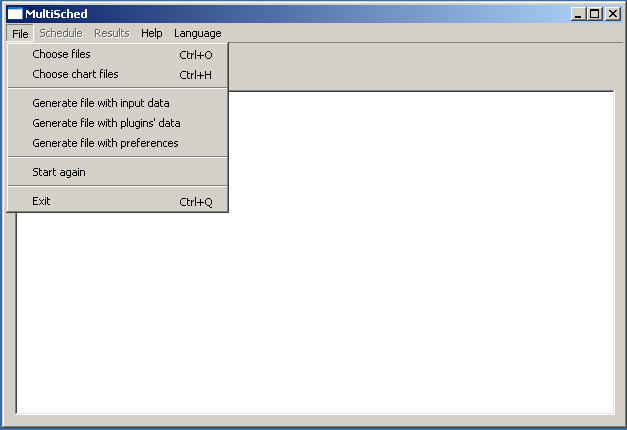
\includegraphics[scale=0.8]{figures/screens/menu_file.png}
\caption{Okno główne -- menu \emph{File}.}\label{rys:mainwindow}
\end{figure}

\subsection{Przykładowe wykonanie głównej ścieżki programu}

Po wybraniu z menu \emph{File} opcji \emph{Choose files} pokazuje się okno wyboru plików wejściowych dla uszeregowania (rys.~\vref{rys:choose_files}).
Ścieżkę do pliku można wpisać bezpośrednio lub skorzystać z przycisku \emph{Browse}. Powoduje on wyświetlenie 
standardowego dialogu otwarcia pliku (wykorzystano tu klasę \code{QFileDialog} oraz jej metodę statyczną \code{getOpenFileName}, która zwraca 
nam łańcuch tekstowy będący ścieżką do wybranego pliku). Wybór plików można zaakceptować przyciskiem \emph{Ok} lub odrzucić -- \emph{Cancel}.

\begin{figure}[htp]
\centering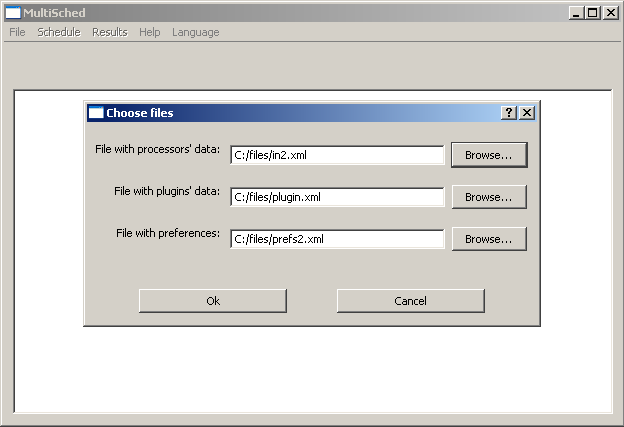
\includegraphics[scale=0.8]{figures/screens/choose_files.png}
\caption{Okno wyboru plików wejściowych.}\label{rys:choose_files}
\end{figure}

Zatwierdzenie opisanego wyżej dialogu powoduje wypisanie w obszarze tekstowym aktualnych ścieżek do plików wybranych przez użytkownika jako stanowiące 
wejście do programu. Jednocześnie w menu uaktywnia się opcja \emph{Choose plugin} w podmenu \emph{Schedule} (rys.~\vref{rys:read_files} oraz 
\vref{rys:menu_schedule}).

\begin{figure}[htp]
\centering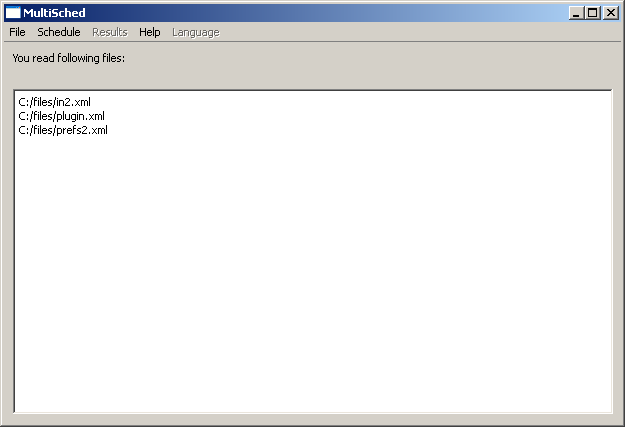
\includegraphics[scale=0.8]{figures/screens/read_files.png}
\caption{Wczytane ścieżki do plików wejściowych.}\label{rys:read_files}
\end{figure}

\begin{figure}[htp]
\centering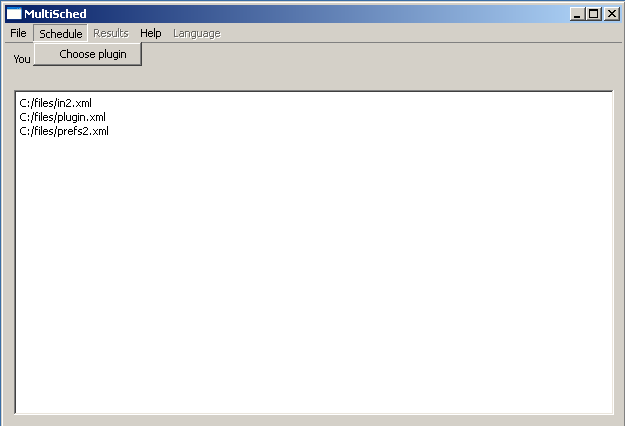
\includegraphics[scale=0.8]{figures/screens/menu_schedule.png}
\caption{Menu \emph{Schedule}.}\label{rys:menu_schedule}
\end{figure}

Dopiero użycie opcji \emph{Choose plugin} powoduje rzeczywiste wczytanie plików, ich walidację i weryfikację zawartych w nich danych. Na podstawie 
zawartości plików wyświetlane są algorytmy dostępne w programie. Użytkownik ma możliwość wybrania jednego z nich (rys.~\vref{rys:choose_plugin}). Za pomocą 
przycisku \emph{Schedule} znajdującego się po prawej stronie rozwijanej listy wyboru uruchamiana jest dla danej wtyczki metoda znajdująca uszeregowanie 
dla wczytanych danych wejściowych.

\begin{figure}[htp]
\centering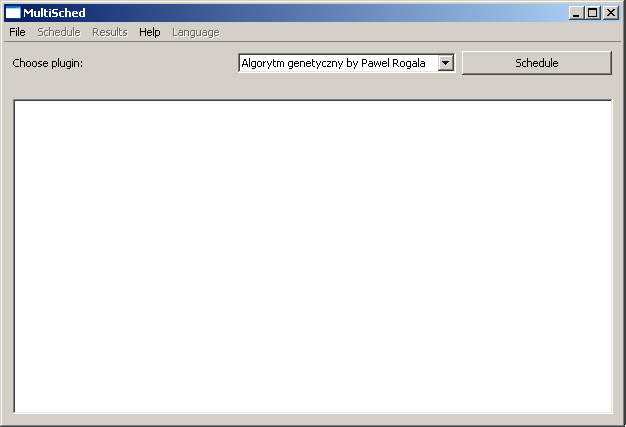
\includegraphics[scale=0.8]{figures/screens/choose_plugin.png}
\caption{Wybór wtyczki szeregującej zadania.}\label{rys:choose_plugin}
\end{figure}

Po znalezieniu uszeregowania uaktywnione zostają opcje w menu \emph{Results} (rys.~\vref{rys:menu_results}). 
Jeśli algorytm nie znalazł rozwiązania, wyświetlona jest tylko informacja, natomiast menu pozostaje nieaktywne.

\begin{figure}[htp]
\centering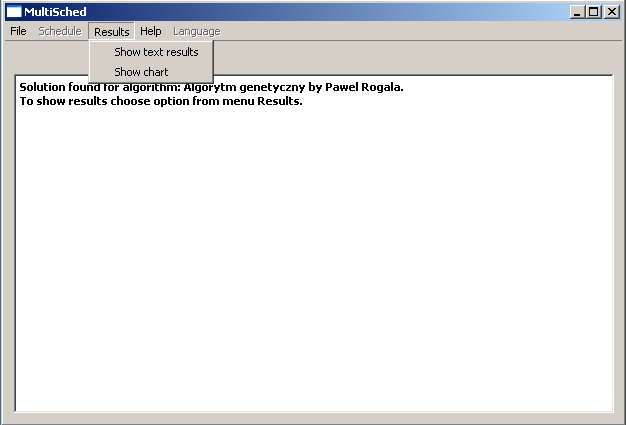
\includegraphics[scale=0.8]{figures/screens/menu_results.png}
\caption{Menu \emph{Results}.}\label{rys:menu_results}
\end{figure}

Menu \emph{Results} oferuje użytkownikowi 2 dostępne opcje:
\begin{itemize}
	\item \textbf{Show text results} -- wybranie tej opcji sprawia, że wyświetlone zostaje okno z wynikami działania algorytmu (rys.~\vref{rys:text_results1} 
	oraz \vref{rys:text_results2}). Główną część okna stanowi obszar tekstowy prezentujący rezultaty. Oprócz znalezionego uszeregowania podawane są 
	takie informacje jak np.~$C_{max}$, dane o obliczeniach (czas, pośrednie wyniki), informacje o działaniu algorytmu 
	genetycznego. Dostęp do funkcji zapisu wyników do pliku tekstowego oraz XML jest zrealizowany za pomocą dwóch z przycisków umieszczonych w dolnej 
	części dialogu (opcje: \emph{Save results as text} oraz \emph{Save schedule as XML}). Funkcje obsługujące te przyciski wykorzystują 
	klasę \code{QFileDialog} a z niej metodę statyczną \code{getSaveFileName}, zwracającą tekst będący ścieżką do pliku, który ma zostać zapisany. 
	Trzeci z przycisków powoduje zamknięcie okna z wynikami.
	\item \textbf{Show chart} -- wybór tej funkcji powoduje wyświetlenie okna z wykresem Gantta wygenerowanym na podstawie wyników działania algorytmu 
	szeregującego (rys.~\vref{rys:chart_results1} oraz \vref{rys:chart_results2}). Obszar wykresu jest umieszczony w centralnej części okna. 
	Jeśli jego rozmiar jest większy niż okno wyświetlające rezultaty graficzne, obok obrazka pojawiają się paski przewijania umożliwiające 
	jego przesuwanie. Możliwa jest też zmiana wymiarów okna, tak aby cały wykres był widoczny na ekranie. Przycisk \emph{Save as jpg image} 
	wywołuje metodę zapisu wykresu do pliku graficznego w formacie JPG. 
\end{itemize}

\begin{figure}[htp]
\centering 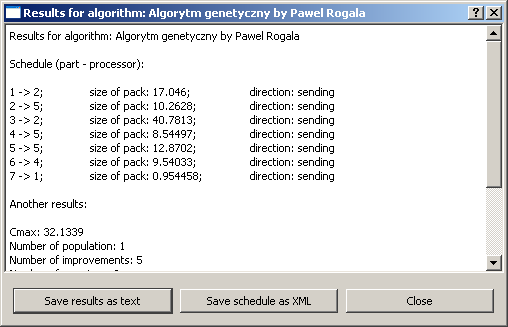
\includegraphics[scale=1]{figures/screens/text_results1.png}
\caption{Tekstowe rezultaty wykonania algorytmu -- 1.}\label{rys:text_results1}
\end{figure}

\begin{figure}[htp]
\centering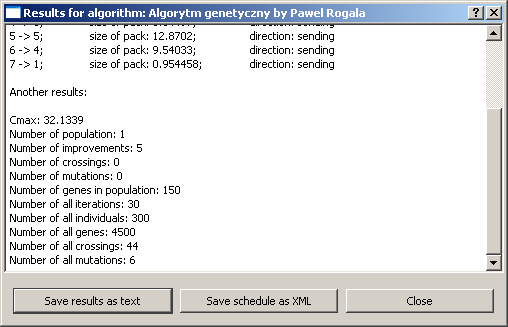
\includegraphics[scale=1]{figures/screens/text_results2.png}
\caption{Tekstowe rezultaty wykonania algorytmu -- 2.}\label{rys:text_results2}
\end{figure}

\begin{figure}[htp]
\centering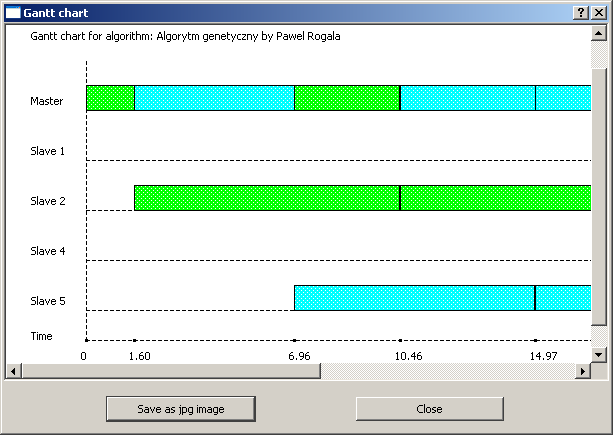
\includegraphics[scale=0.75]{figures/screens/chart_results1.png}
\caption{Graficzne rezultaty wykonania algorytmu -- wykres Gantta -- 1.}\label{rys:chart_results1}
\end{figure}

\begin{figure}[htp]
\centering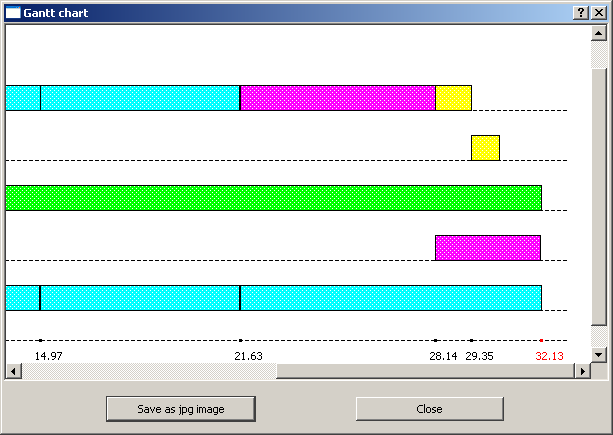
\includegraphics[scale=0.75]{figures/screens/chart_results2.png}
\caption{Graficzne rezultaty wykonania algorytmu -- wykres Gantta -- 2.}\label{rys:chart_results2}
\end{figure}

\subsection*{Wygląd interfejsu podczas generowania wykresu na podstawie gotowego uszeregowania}

Kolejną dostępną opcją w menu \emph{File} jest funkcja \emph{Choose chart files} (rys.~\vref{rys:choose_chart_files}). 
Dzięki niej użytkownik ma możliwość narysowania wykresu Gantta na podstawie gotowego uszeregowania podanego w postaci pliku XML oraz informacji o procesorach. 
Wybranie plików powoduje uaktywnienie opcji \emph{Show chart} z menu \emph{Results}. Jednak w tym przypadku opcja ta sprawi, że przed narysowaniem wykresu 
zostanie zweryfikowana poprawność plików XML oraz ich dopasowanie do siebie (m.in pod kątem wykorzystanych procesorów).

\begin{figure}[htp]
\centering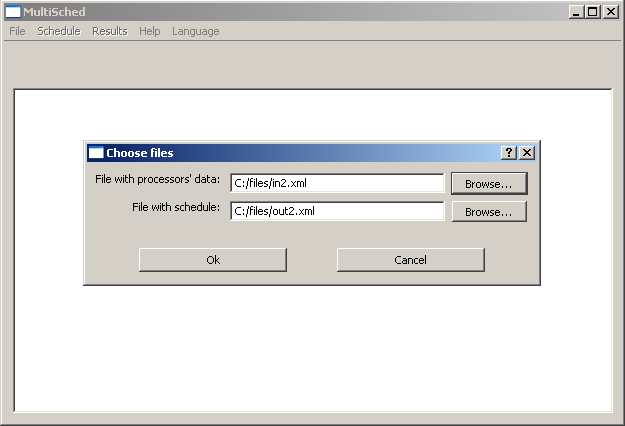
\includegraphics[scale=0.8]{figures/screens/choose_chart_files.png}
\caption{Okno wyboru plików potrzebnych do narysowania wykresu na podstawie gotowego uszeregowania.}\label{rys:choose_chart_files}
\end{figure}

\subsection{Pozostałe funkcje menu}

Następną grupę funkcji w menu \emph{File} stanowią możliwości uruchomienia kreatorów (\english{wizard}) tworzenia plików wejściowych. Użytkownik ma do wyboru trzy 
kreatory: 
\begin{itemize}
	\item Kreator plików z informacjami o wolumenie danych, procesorach, liczbie zadań i paczek oraz z danymi dla algorytmu genetycznego.
	\item Kreator plików z danymi wtyczek dostępnych w systemie.
	\item Kreator plików zawierających preferencje użytkownika.
\end{itemize}

Każda klasa kreatora dziedziczy z tej samej nadklasy (\code{SimpleWizard}) i dlatego wygląd takiego okna jest ujednolicony. U dołu każdej strony 
znajdują się następujące przyciski:
\begin{itemize}
	\item \textbf{Cancel} -- anulowanie tworzenia pliku,
	\item \textbf{Back} -- powrót do poprzedniej strony kreatora (nieaktywny w przypadku pierwszej strony),
	\item \textbf{Next} -- przejście do następnej strony kreatora (nieaktywny w przypadku ostatniej strony)
	\item \textbf{Finish} -- zatwierdzenie wszystkich wprowadzonych danych (uaktywnia się na ostatniej stronie). Po naciśnięciu przycisku dokonywana 
	jest ostateczna weryfikacja podanych wartości. Jeśli są one poprawne, wyświetlany jest standardowy dialog zapisu pliku.
\end{itemize}

Reszta kontrolek na każdej stronie kreatora zależy od jego rodzaju:

\subsubsection*{Kreator pliku z danymi wejściowymi dla algorytmu szeregującego zadania}

Pierwszą stronę opisywanego wizarda przedstawia rys.~\vref{rys:generate1_1}. Na stronie tej użytkownik podaje 
ogólne informacje dotyczące danych wejściowych takie jak: rozmiar wolumenu danych, liczba zadań do wykonania, liczba paczek, na jakie ma być podzielony 
wolumen, oraz całkowita liczba procesorów przetwarzających. Po wypełnieniu wszystkich wartości z pierwszego formularza możliwe staje się przejście do następnej strony 
(rys.~\vref{rys:generate1_2}). Wartości wprowadzane do kolejnego formularza dotyczą procesorów przetwarzających. 
Dla każdej maszyny należy podać takie dane jak: koszt użycia, prędkość przetwarzania, prędkość komunikacji łącza między nadzorcą a procesorami 
roboczymi, opóźnienie startowe łącza (\english{startup time}) oraz pojemność bufora pamięciowego. Wykorzystano tutaj klasę \code{QTableWidget}. 
Dzięki temu możliwe jest dynamiczne tworzenie liczby pól służących do wprowadzania wartości w zależności od podanej na pierwszej stronie liczby 
procesorów. Na stronie trzeciej (rys.~\vref{rys:generate1_3}) możliwy jest wybór opcji podania parametrów wejściowych dla algorytmu genetycznego. 
W zależności od tego czy opcja ta została zaznaczona, uaktywnia się lub dezaktywuje zbiór kontrolek, za 
pomocą których należy wprowadzić wartości opisane wyżej w rozdziale~\vref{pliki}. Po wypełnieniu (lub wybraniu) wymaganych wartości formularz 
może zostać zatwierdzony.

\begin{figure}[htp]
\centering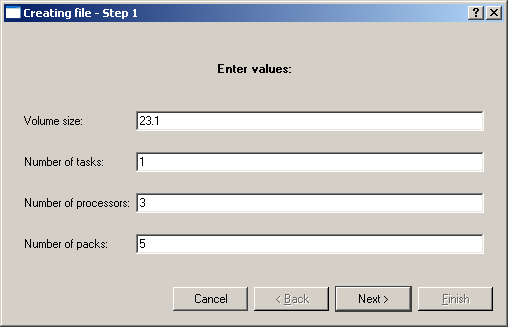
\includegraphics[scale=0.7]{figures/screens/generate1_1.png}
\caption{Kreator pliku wejściowego -- strona 1.}\label{rys:generate1_1}
\end{figure}

\begin{figure}[htp]
\centering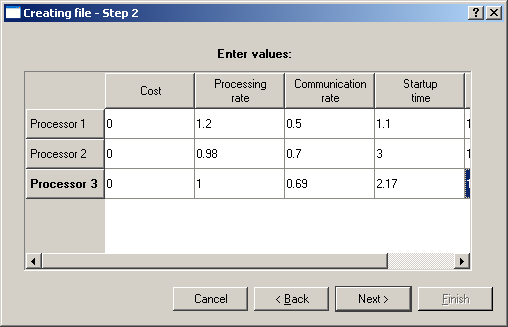
\includegraphics[scale=0.7]{figures/screens/generate1_2.png}
\caption{Kreator pliku wejściowego -- strona 2.}\label{rys:generate1_2}
\end{figure}

\begin{figure}[t]
\centering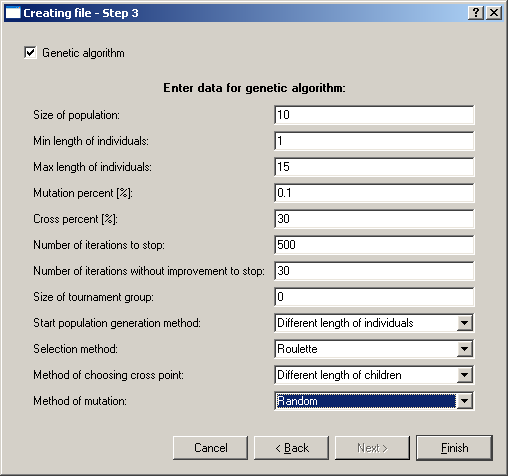
\includegraphics[scale=0.65]{figures/screens/generate1_3.png}
\caption{Kreator pliku wejściowego -- strona 3.}\label{rys:generate1_3}
\end{figure}

\subsubsection*{Kreator pliku z danymi wtyczek dostępnych w systemie}

Pierwszy formularz wizarda zawiera tylko jedno pole tekstowe, w które należy wprowadzić liczbę algorytmów, których dane ma zawierać plik 
(rys.~\vref{rys:generate2_1}). Po wprowadzeniu poprawnej liczby możliwe jest przejście do drugiej strony 
(rys.~\vref{rys:generate2_2_1} oraz \vref{rys:generate2_2_2}). Na niej w zależności od podanej wcześniej liczby wyświetlana jest odpowiedniej wielkości 
tabela, w której dla każdej wtyczki użytkownik musi podać następujące informacje: nazwa, autor, krótki opis, typ (algorytm dokładny lub heurystyka) 
i ewentualnie podtyp (np.~algorytm genetyczny), czy następuje zwracanie wyników do inicjatora oraz ograniczenia pamięciowe, a także ścieżkę dostępu 
do pliku z wtyczką (biblioteki łączonej dynamicznie). Po podaniu wszystkich wartości formularz może zostać zatwierdzony.

\begin{figure}[htp]
\centering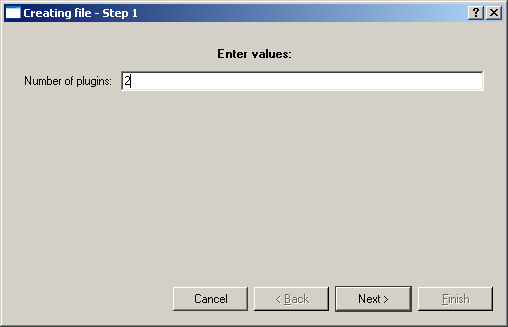
\includegraphics[scale=0.7]{figures/screens/generate2_1.png}
\caption{Kreator pliku z danymi wtyczek -- strona 1.}\label{rys:generate2_1}
\end{figure}

\begin{figure}[htp]
\centering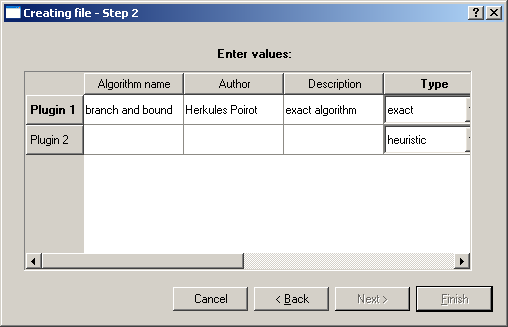
\includegraphics[scale=0.7]{figures/screens/generate2_2_1.png}
\caption{Kreator pliku z danymi wtyczek -- strona 2.}\label{rys:generate2_2_1}
\end{figure}

\begin{figure}[htp]
\centering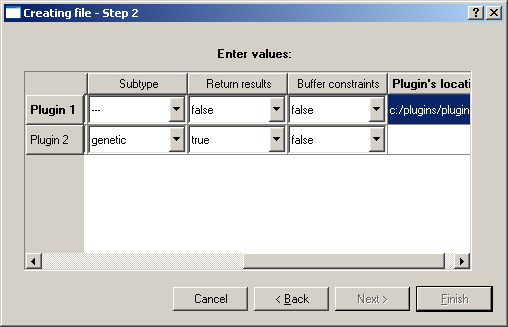
\includegraphics[scale=0.7]{figures/screens/generate2_2_2.png}
\caption{Kreator pliku z danymi wtyczek -- strona 2.}\label{rys:generate2_2_2}
\end{figure}

\subsubsection*{Kreator pliku z preferencjami użytkownika}

Kreator ten składa się z jednej strony (rys.~\vref{rys:generate3}). Za pomocą rozwijanych list wyboru użytkownik 
może podać swoje preferencje dotyczące wykonywanego algorytmu. Po zatwierdzeniu strony wprowadzone wartości zapisywane są do pliku XML o wybranej 
nazwie i lokalizacji.

\begin{figure}[htp]
\centering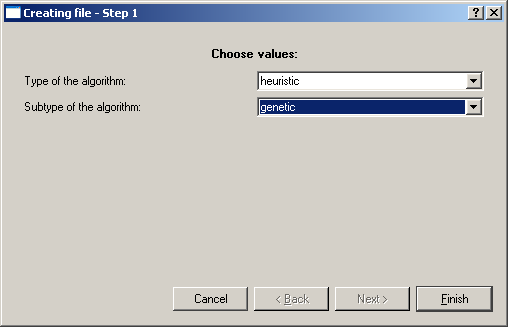
\includegraphics[scale=0.7]{figures/screens/generate3.png}
\caption{Kreator pliku z preferencjami użytkownika.}\label{rys:generate3}
\end{figure}

\subsubsection*{Start again}

Opcja ta jest dostępna z poziomu menu \emph{File}. Jej wybranie powoduje wyzerowanie wartości wszystkich zmiennych i zmianę stanu aplikacji na 
taki jaki występuje bezpośrednio po uruchomieniu. Opcję tę należy wybrać, jeśli po wykonaniu jakiejś ścieżki programu użytkownik chce wykonać 
kolejną.

\subsubsection*{Menu Help}
Menu \emph{Help} zawiera opcje wyświetlenia pomocy jako pliku w formacie Windows Help (z rozdzerzeniem \texttt{chm}) a także informacji 
o programie MultiSched.

\subsubsection*{Menu Language}
Menu \emph{Language} umożliwia zmianę języka interfejsu aplikacji (na polski -- gdy program działał w wersji angielskiej i odwrotnie).

\subsection{Opis przykładu}

Wyniki tekstowe oraz graficzne zamieszczone na rysunkach \vref{rys:text_results1}, \vref{rys:text_results2}, \vref{rys:chart_results1} oraz 
\vref{rys:chart_results2} ilustrują działanie algorytmu genetycznego dla przykładowego pliku wejściowego zamieszczonego na stronie \pageref{lst1}. 
Analizując wartości zawarte w tym pliku, można zrozumieć dlaczego poszczególne części zostały przyporządkowane do takich a nie innych procesorów 
przetwarzających. Jak widać z wykresu najwięcej części jest przydzielonych do procesorów nr 2 oraz 5. Łatwo zauważyć, że właśnie te maszyny charakteryzują 
się najmniejszym opóźnieniem startowym łącz oraz najwiekszą prędkością przesyłania danych. Procesor nr 4 ma co prawda również nie najgorsze parametry 
takie jak prędkość łącza i przetwarzania, jednak wysoka wartość opóźnienia startowego powoduje, że w znalezionym uszeregowaniu przyporządkowana 
jest do niego tylko jedna paczka danych.

\chapter{Testowanie poprawności działania programu}

Każdy program, aby mógł być wykorzystywany zgodnie z przeznaczeniem, musi zapewniać poprawność działania. W tym celu niezbędne jest jego zabezpieczenie 
przed wszelkimi błędami jakie mogą wystąpić i gruntowne przetestowanie. Najczęstsze nieprawidłowości w działaniu jakie mogłyby się zdarzyć podczas 
użytkowania związane są z błędnymi danymi, które podałby użytkownik. Dlatego też w aplikacji MultiSched duży nacisk został położony na wszechstronną 
weryfikację poprawności wszelkich wartości stanowiących dane wejściowe poszczególnych funkcji aplikacji.

Sprawdzanie poprawności rozpoczyna się już na początku działania programu. Podczas wczytywania plików wejściowych pierwszym zabezpieczeniem 
jest sprawdzenie czy podane przez użytkownika ścieżki odpowiadają rzeczywistym plikom istniejącym fizycznie na dysku. Jeśli tak, to wywoływane są 
funkcje wczytujące pliki XML do obiektów. W przypadku, gdy plik nie istnieje albo zostanie napotkany błąd w pliku (np.~nieistniejący znacznik czy 
też zły typ lub zakres wartości) użytkownikowi wyświetlone zostaje okno z komunikatem ostrzegającym o błędzie. Za walidację plików XML odpowiadają 
metody z klasy \code{Reader}. Sprawdzenie poprawności znaczników następuje równolegle z parsowaniem pliku -- wykrycie nieprawidłowości od razu 
powoduje zakończenie dalszego przetwarzania. Natomiast za weryfikację odczytanych wartości i porównanie ich z zasadami zdefiniowanymi w XML Schema 
odpowiedzialne są funkcje \code{bool Reader::verifyData(Data *data)} oraz \code{bool Reader::verifyChartData(ChartData *data)}. Opisane czynności 
są wykonywane zarówno podczas wczytywania plików z danymi wejściowymi do algorytmów szeregujących jak i plików z gotowym uszeregowaniem będących 
podstawą do wygenerowania wykresu Gantta.

Przy ładowaniu pliku z parametrami procesorów oraz danymi wejściowymi dla algorytmów genetycznych wartości sprawdzane są pod następującym kątem:
\begin{itemize}
	\item rozmiar wolumenu danych -- może stanowić dodatnią wartość liczbową;
	\item liczba procesorów, paczek i zadań -- to wartości dodatnie całkowitoliczbowe (integer);
	\item koszt użycia procesora, rozmiar bufora oraz opóźnienie startowe -- liczby nieujemne;
	\item odwrotności prędkości przetwarzania oraz komunikacji -- muszą być wartościami dodatnimi;
	\item rozmiar populacji, minimalna i maksymalna długość osobnika, maksymalna liczba iteracji algorytmu genetycznego -- 
		opisane są przez liczby całkowite dodatnie;
	\item prawdopodobieństwo krzyżowania oraz mutacji -- podawane są w procentach, więc mogą być określone przez liczby zmiennoprzecinkowe 
		z przedziału $\langle$0, 100$\rangle$;
	\item rozmiar grupy turniejowej -- wartość ta musi być większa lub równa 0, całkowitoliczbowa;
	\item metoda generacji populacji startowej -- może wynosić 0 (różna długość osobników) lub 1 (jednakowa długość osobników);
	\item metody: selekcji, mutacji oraz wyboru punktu krzyżowania -- przyjmują wartości 1 lub 2.
\end{itemize}

Wartości w pliku z informacjami o wtyczkach dostępnych w systemie mogą być następujące:
\begin{itemize}
	\item autor, nazwa i opis algorytmu a także lokalizacja wtyczki -- łańcuchy znaków;
	\item informacja o zwracaniu wyników oraz ograniczeniach pamięciowych -- przyjmuje wartości \code{true} lub \code{false};
	\item\label{typ-algo} typ algorytmu -- może być zdefiniowany jako \code{exact} albo \code{heuristic}, a podtyp jako \code{genetic} lub \code{other};
\end{itemize}

Plik opisujący preferencje użytkownika dotyczące algorytmu może zawierać wartości opisane powyżej w punkcie~\vref{typ-algo}.

Dane w dokumencie zawierającym gotowe uszeregowanie (czyli najczęściej pliku wyjściowym będącym rezultatem działania którejś z wtyczek) umieszczone 
powinny być z zachowaniem następujących zasad zakresów wartości:
\begin{itemize}
	\item identyfikator paczki oraz identyfikator procesora -- liczba dodatnia, całkowita;
	\item rozmiar paczki -- liczba dodatnia;
	\item kierunek przesyłania paczki -- \emph{sending} lub \emph{receipt};
\end{itemize}

Kolejne sprawdzanie poprawności danych jest wykonywane podczas wczytywania wybranej przez użytkownika wtyczki. Funkcja ładująca sprawdza najpierw 
czy lokalizacja wpisana przez użytkownika w pliku z opisem algorytmów jest właściwą ścieżką do pliku. Gdy okazuje się, że jest ona nieprawidłowa, 
użytkownik jest o tym informowany komunikatem. I podobnie -- ostrzeżenie o błędzie wyświetla się, w przypadku kiedy wskazywany przez ścieżkę plik 
nie jest prawidłową biblioteką łączoną dynamicznie i nie można go załadować i użyć w programie.

Weryfikacja podawanych przez użytkownika wartości jest niezbędna również podczas tworzenia plików za pomocą kreatorów. Tam na każdym etapie 
po wypełnieniu wszystkich wymaganych pól przy próbie przejścia do nowej strony lub zatwierdzenia działania kreatora wywoływane są metody walidujące.
Zasady sprawdzania wartości, które wprowadził  użytkownik są identyczne jak przy weryfikacji poprawności wczytywanych plików wejściowych.
Jak w każdym przypadku, po wystąpieniu błędu wyświetlany jest odpowiednie okno komunikatu z informacją dla użytkownika. Dzięki takiemu podejściu 
użytkownik ma pewność, że stworzone przez niego pliki są zgodne z określonymi dla nich dokumentami XML Schema.

\chapter{Podsumowanie}

%Tekst o tym jakie to fajne jest przetwarzanie równoległe
Celem pracy było stworzenie systemu do oceny i porównywania algorytmów szeregowania zadań jednorodnych. Motywacją dla takiej pracy jest 
coraz większa popularność sieci komputerowych i przetwarzania równoległego a przez to konieczność wyboru odpowiedniej metody realizacji 
takiego przetwarzania dostosowanej do istniejących warunków. W ramach realizacji zadania powstała aplikacja \emph{MultiSched} umożliwiająca 
znalezienie rozwiązania problemu szeregowania za pomocą różnych algorytmów wybieranych przez użytkownika. Program ten udostępnia użytkownikowi 
szereg funkcji, dzięki którym może znaleźć szerokie zastosowanie w analizie problemu szeregowania zadań jednorodnych oraz algorytmów służących 
do jego rozwiązywania. Na uwagę zasługuje możliwość rozszerzenia funkcjonalności aplikacji o analizę kolejnych algorytmów poprzez opcję 
łatwego dołączania wtyczek jako bibliotek łączonych dynamicznie. W programie zastosowano ogólny format danych, który można zaadaptować do wielu 
specyficznych problemów szeregowania zadań jednorodnych. Poprawność działania programu została zapewniona poprzez szczegółową analizę 
wprowadzanych przez użytkownika danych wejściowych i odporność na próby podania nieprawidłowych wartości.
Warto rozważyć rozszerzenie aplikacji o nowe wtyczki implementujące kolejne algorytmy szeregowania zadań jednorodnych. Większa liczba takich 
wtyczek dawałaby szansę na bardziej szczegółowe porównanie ich działania oraz możliwość lepszego wyboru konkretnego algorytmu dla wybranych 
zastosowań w świecie rzeczywistym.

